\documentclass[12pt,a4paper]{article}

\usepackage[OT1]{fontenc}
\usepackage[utf8]{inputenc}
\usepackage[russian,english]{babel}
%%%% Additional part of preamble generated by package Sweave in RStudio
%% initial declaration for fonts
\usepackage[labelfont=bf]{caption}
\usepackage[font=small,labelfont=bf]{subcaption}


%% For tables
\usepackage{array}
\usepackage{longtable}
\usepackage{fullpage}
\usepackage{dcolumn}
\usepackage[flushleft]{threeparttable}
\usepackage{booktabs}
\usepackage[12hr]{datetime}
\usepackage[DIV=16]{typearea}
\usepackage{scrextend,booktabs}
\usepackage{tabulary}
\usepackage{multirow}
\usepackage[font=footnotesize]{caption}


%% Additional elements for figures and numbering added by Sweave
\usepackage{float}
\usepackage[sc]{mathpazo}
\usepackage{geometry}
\geometry{verbose,tmargin=2.5cm,bmargin=2.5cm,lmargin=2.5cm,rmargin=2.5cm}
\setcounter{secnumdepth}{2}
\setcounter{tocdepth}{2}
\usepackage{url}


%% Additional links for hyperref
\usepackage[unicode=true,pdfusetitle,
 bookmarks=true,bookmarksnumbered=true,bookmarksopen=true,bookmarksopenlevel=2,
 breaklinks=false,pdfborder={0 0 1},backref=false,colorlinks=false]
 {hyperref}
\hypersetup{
 pdfstartview={XYZ null null 1}}

\usepackage{breakurl}
\usepackage{Sweave}


\usepackage[backend=bibtex,
                style=authoryear,
                natbib=true, 
                style=authoryear]{biblatex}
\addbibresource{Returns.bib}

\DefineBibliographyStrings{russian}{%
  bibliography = {References},
  references={References} 
}



\begin{document}


\title{Working Paper 1: Returns to Education in the Russian Federation - Zeroth Draft \footnote{Arranged in alphabetical order of author last names. The entire code used to generate the graphs and tables presented in this paper is available on bitbucket at \burl{https://bitbucket.org/zagamog/edreru/src/master/} , starting from the raw RLMS data graciously provided in the public domain by the National Research University-Higher School of Economics (HSE).}}
\author{Ekaterina Melianova, Suhas D. Parandekar, Harry A. Patrinos, Art\"{e}m Volgin}
\maketitle
\begin{abstract}
This is the first cut at Working Paper 1 (of proposed 3 working papers) on the Returns of Education in the Russian Federation. The paper shows an interesting pattern of variation in the returns to education from 1994-2018. The paper shows the co-movement of returns to higher education and the return to vocational education. From a policy viewpoint, it shows that returns to education may be strongly influencing decisions of individuals or families regarding their future education trajectories. Policy initiatives seeking to influence enrollment trends at specific educational levels would need to consider the empirical antecedents. 
\end{abstract}


\section*{RLMS Results}

\subsection*{Data}

To estimate returns to education in Russia we employed the Russian Longitudinal 
Monitoring Survey (RLMS) - the longest panel survey of individuals and 
households in Eastern Europe and Asia and the only representative Russian 
survey with a sizable panel component allowing for a dynamic analysis 
\parencite{kozyreva_081._2015}. The data are notable for their reliability, 
diversity, and applicability to a variety of research questions. The RLMS 
embraces information on people's income and expenditure structure, their 
material well-being, educational and occupational behavior, health state and 
nutrition, migration, etc.  RLMS sampling procedures have been thoroughly and 
extensively described elsewhere \parencite{kozyreva_081._2015}. The present 
research uses all 23 waves (1994 - 2018) that are available as of \today. The 
sub-sample selected for empirical investigation  in this paper consists of 
working individuals aged 25-64 who are out of school and have positive labor 
market experience and income.
\\

\subsection*{Methods}

Our empirical analysis pertains to the examination of a slightly modified basic specification of a mincer-type wage equation \parencite{mincer_082._1974}. We present results for the general working population of the Russian Federation aged 25-64 as well as by gender and nationality. The specification of focus is as follows:

$$Log(Wage) = b_0 + b_1\cdot Educ + b_2\cdot Exp + b_3\cdot Exp^2 + b_4\cdot Gender + b_5\cdot Nationality + \epsilon$$

where $Log(Wage)$ is a logarithm of monthly wage, $Educ$ stands for the highest attained level of education, $Exp$ and $Exp^2$ reflect the years of working experience and its quadratic term respectively, $Gender$ is a dummy variable for gender, $Nationality$ represents a person's nationality, $b_0$ is an intercept, $b_1 ... b_n$ are the respective slope estimates, $\epsilon$ refers to a normally distributed error term.
\\

\subsection*{Measures}

\subsubsection*{Dependent variable}

For the dependent variable we used the logarithm of an average monthly wage within the past year on a person's primary job (J13.2 variable in the RLMS dataset). If a person had an additional job, the maximum wage value among the two (J13.2 and J40) was selected for the analysis. In the waves from 1994 to 1996 the above mentioned question was absent; for those waves we exploited a variable about the average amount of money earned by a respondent within the past 30 days (J10) as a reasonable approximation.
\\

\subsubsection*{Independent variables}

We distinguished 3 categories for the {\bf education} variable (EDUC): (1) secondary, (2) vocational, and (3) higher. Incomplete levels were incorporated into the respective upper categories (e.g., incomplete higher - into higher). We are interested in exploring returns to vocational and higher education. Estimations of premiums to primary and secondary schooling levels are technically unreachable to us since the number of adults without primary education and the number of adults with only primary level are minuscule in the general population. 
\\

\subsection*{Construction of experience variable}

Absence of data regarding a person's actual experience profile often compels researchers to employ a heuristic such as experience is equal to age less the official age of entrance into school and less the duration of schooling in years. However, this method introduces measurement error that drives imprecision in results, especially important if we want to compare changes in the rate of returns to education over time. Fortunately,  RLMS is a panel data with most individuals surveyed over multiple years, which allows the creation of a factual experience variable. There is considerable attrition in the data over time, with like for like replacements of households to maintain national representativeness of the sample. RLMS also follows the somewhat innovative practice of continuing to sample a dwelling if the household residing in the dwelling has moved away; a sampling practice which implies an increasing sample size over time. Another implication of the sampling scheme is that computing labor market experience is a bit complicated and necessitates some assumptions and imputations that are explained below. \\


To create a variable displaying a person's {\bf experience} we leveraged four questions on the year and a month of starting the primary job and the month of starting an additional job, if applicable (J5A, J5B, J35.2Y, and J25.2M). Based on these variables and the information of the interview date, a labor market experience variable was generated for each unique respondent in the sample by summing up his or her experience registered \textit{across} RLMS waves. If an employed individual had missing values on a date of his or her start of work in a particular survey year, and the individual had appeared at any time in a previous year, the first non-missing record from previous waves was chosen. If only the year of a job start was provided, we standardized computation by imputing the month to be January of that year. In cases of the absence of a valid answer with regard to both year and month of job start in both primary and additional job in all RLMS waves a person was surveyed, such cases (< 1\%) were dropped from the analysis. List-wise deletion strategy was also applied to the observations with "negative" experience (< 1\%) when according to one's responses a job started allegedly "after" the interview occurred\footnote{This step is necessitated because of the mixed panel nature of RLMS. Without proper accounting of experience, with education at a fixed level and changing income for an individuala cross years, there would be avoidable noise and possibly bias introduced on the education coefficient in the Mincerian equation.} 
\\

A routine was therefore elaborated for detecting and fixing inconsistent responses to the questions about experience. The `quality control' on the experience variable revealed two opposing apparent recollection errors:

\begin{enumerate}
\item individuals whose starting date of a first job became at a later date over successive waves (e.g., an individual said in 2001 that she started working in 2000; the same individual in 2005 said she started working in 2002); 

\item individuals, naming an earlier job starting date compared to the mentioned preceding dates (e.g., a respondent in 2005 said he had started to work in 2000, but in 2001 he or she replied 1995 had been in fact the beginning year of his or her working activity). 
\end{enumerate}

Ideally, people would have perfect recall and not give inconsistent responses about their job history over time. However, we found inconsistent responses for 52\% of unique respondents or 40\% of instances in the pooled RLMS database (1994 - 2018).In both situations (whether computed experience increased or decreased due to different recollections of start date of first job), the  routine used in this paper prioritizes earlier responses, based on the reasoning that memory fades over time.  The method used in this paper is not able to eliminate the error, but dealing with it in a consistent manner appears a better approach than simply imputing an experience variable assuming a person started working since finishing education and has been working ever since.\\



Table 1 shows the results of averaging all the three ways of generating labor market experience by cohorts of respondents aggregated on the basis of the number of incidences in the RLMS survey. The first column shows that there were 6667 individuals who appeared only once in the RLMS, 3463 who appeared twice (though could have been different pairs of years), 2793 who appeared three times and so on until the 119 individuals who appeared 23 times in the survey. Table 1 shows the mean values of the experience variable in years as computed by three methods: (EX1) The method outlined above, chosing earliest available data in case of inconsistencies; (EX2) method looking at each year of data independently, ignoring any inconsistencies, and (EX3) Na\"ive estimates which is simply the age - duration of schooling - 6.\\

The table demonstrates that the two corresponding versions of experience computed with (EX1) and without (EX2) inconsistency correction gradually increase with the rise of the number of instances an individual appeared in RLMS. These differeces are mostly statistically significant as can be seen from the displayed p-values for a t-test of no significant difference.  Overall, this indicates the necessity of harmonizing the data in the described manner. 
\\





\begin{table}[H]
\footnotesize
\def\arraystretch{1} 
        \centering
        \caption{Comparison between Initial and Corrected Versions of the Experience Variable}
        \label{tab:1}
% latex table generated in R 3.5.1 by xtable 1.8-4 package
% Thu Oct 31 14:41:07 2019
\begin{tabular}{p{3cm}p{1.5cm}p{1.5cm}p{1.5cm}p{1.5cm}rp{1cm}p{1cm}}
  \hline\hline \\
Cohort - number of  appearances in RLMS & N individuals & Experience correcting error (EX1)  & Experience ignoring error (EX2) & Experience na\"ive (EX3) & N instances & t-tests EX1-EX2: pvalue & t-tests EX1-EX3: pvalue \\ 
  \hline \\
01 & 6667 & 05.91 & 06.25 & 18.91 & 6667 & 0.01 & 0.00 \\ 
    02 & 3463 & 06.53 & 06.97 & 19.26 & 6926 & 0.02 & 0.00 \\ 
    03 & 2793 & 07.60 & 08.10 & 20.41 & 8379 & 0.03 & 0.00 \\ 
    04 & 2556 & 08.41 & 08.90 & 20.35 & 10224 & 0.04 & 0.00 \\ 
    05 & 1729 & 07.99 & 08.82 & 20.35 & 8645 & 0.00 & 0.00 \\ 
    06 & 1532 & 08.56 & 09.43 & 20.02 & 9192 & 0.00 & 0.00 \\ 
    07 & 1273 & 09.41 & 10.36 & 20.45 & 8911 & 0.00 & 0.00 \\ 
    08 & 1177 & 10.14 & 10.88 & 21.13 & 9416 & 0.02 & 0.00 \\ 
    09 & 910 & 10.66 & 11.75 & 21.32 & 8190 & 0.00 & 0.00 \\ 
   10 & 597 & 10.58 & 12.08 & 21.56 & 5970 & 0.00 & 0.00 \\ 
   11 & 541 & 10.52 & 12.04 & 20.85 & 5951 & 0.00 & 0.00 \\ 
   12 & 495 & 11.50 & 12.93 & 22.42 & 5940 & 0.00 & 0.00 \\ 
   13 & 508 & 12.27 & 13.95 & 22.46 & 6604 & 0.00 & 0.00 \\ 
   14 & 325 & 12.63 & 14.10 & 22.47 & 4550 & 0.01 & 0.00 \\ 
   15 & 339 & 13.60 & 15.28 & 22.95 & 5085 & 0.01 & 0.00 \\ 
   16 & 245 & 12.59 & 15.28 & 22.07 & 3920 & 0.00 & 0.00 \\ 
   17 & 235 & 13.77 & 15.99 & 22.91 & 3995 & 0.00 & 0.00 \\ 
   18 & 216 & 14.47 & 15.72 & 22.97 & 3888 & 0.06 & 0.00 \\ 
   19 & 212 & 14.52 & 16.34 & 23.67 & 4028 & 0.00 & 0.00 \\ 
   20 & 153 & 14.97 & 16.84 & 23.06 & 3060 & 0.00 & 0.00 \\ 
   21 &  96 & 16.34 & 17.13 & 25.34 & 2016 & 0.33 & 0.00 \\ 
   22 &  97 & 17.05 & 18.92 & 25.06 & 2134 & 0.04 & 0.00 \\ 
   23 & 119 & 19.63 & 20.88 & 25.87 & 2737 & 0.16 & 0.00 \\ 
   \hline
\end{tabular}
\end{table}


Finally, two socio-demographic variables were incorporated into the analysis, namely gender and nationality. Gender is included in the specification in the form of a dichotomous dummy variable with "1" standing for females, "0" - for males. Nationality is reflected with a 1 if a person did not identify him/herself as Russian and 0 if Russian.

\subsection*{Findings from Estimation of Mincerian Equation}

Figure 1, panel (a) displays rates of returns to higher and vocational education (as compared to secondary education) in Russia in 1994-2018. The results suggest that on average wage premiums to university education in Russia are roughly 3-5 times greater than to vocational schooling. Overall, there is a moderate curved growth in both return types, achieving their peak in the early 2000s (83\% for higher education and 26\% for vocational education compared to the average earnings of workers with the secondary level), which is followed by a downward pattern (see Figure 1). The interesting pattern to note from panel (a) is the apparent co-movement of vocational education and higher education - the higher education smoothing curve turns a bit more sharply than the one for vocational education, but their movement is matching, even at second order levels of smoothness (SP note to team - we need to superimpose with lighter line showing unsmoothed points). Further, even though higher education premium remains much above the premium for vocational education, there is a pereceptible narrowing of the difference in recent years. Panel (b) which is drawn from a presentation made by Marina Telezhkina at the WB-HSE Summer School on the Economics of Education in July 2019, shows the interesting pattern of higher education enrollment rates for population of 17-25 year olds. Figure 1(b) shows the downturn in returns reflected in enrollments, with the peak in enrollments coming about 10 years later. 
\\


\begin{figure}[H]
\caption{\textbf{Rates of Returns to Higher and Vocational Education in Russia, RLMS 1994-2018}}\label{fig1}
         \centering
         \begin{subfigure}[b]{0.5\textwidth}
                 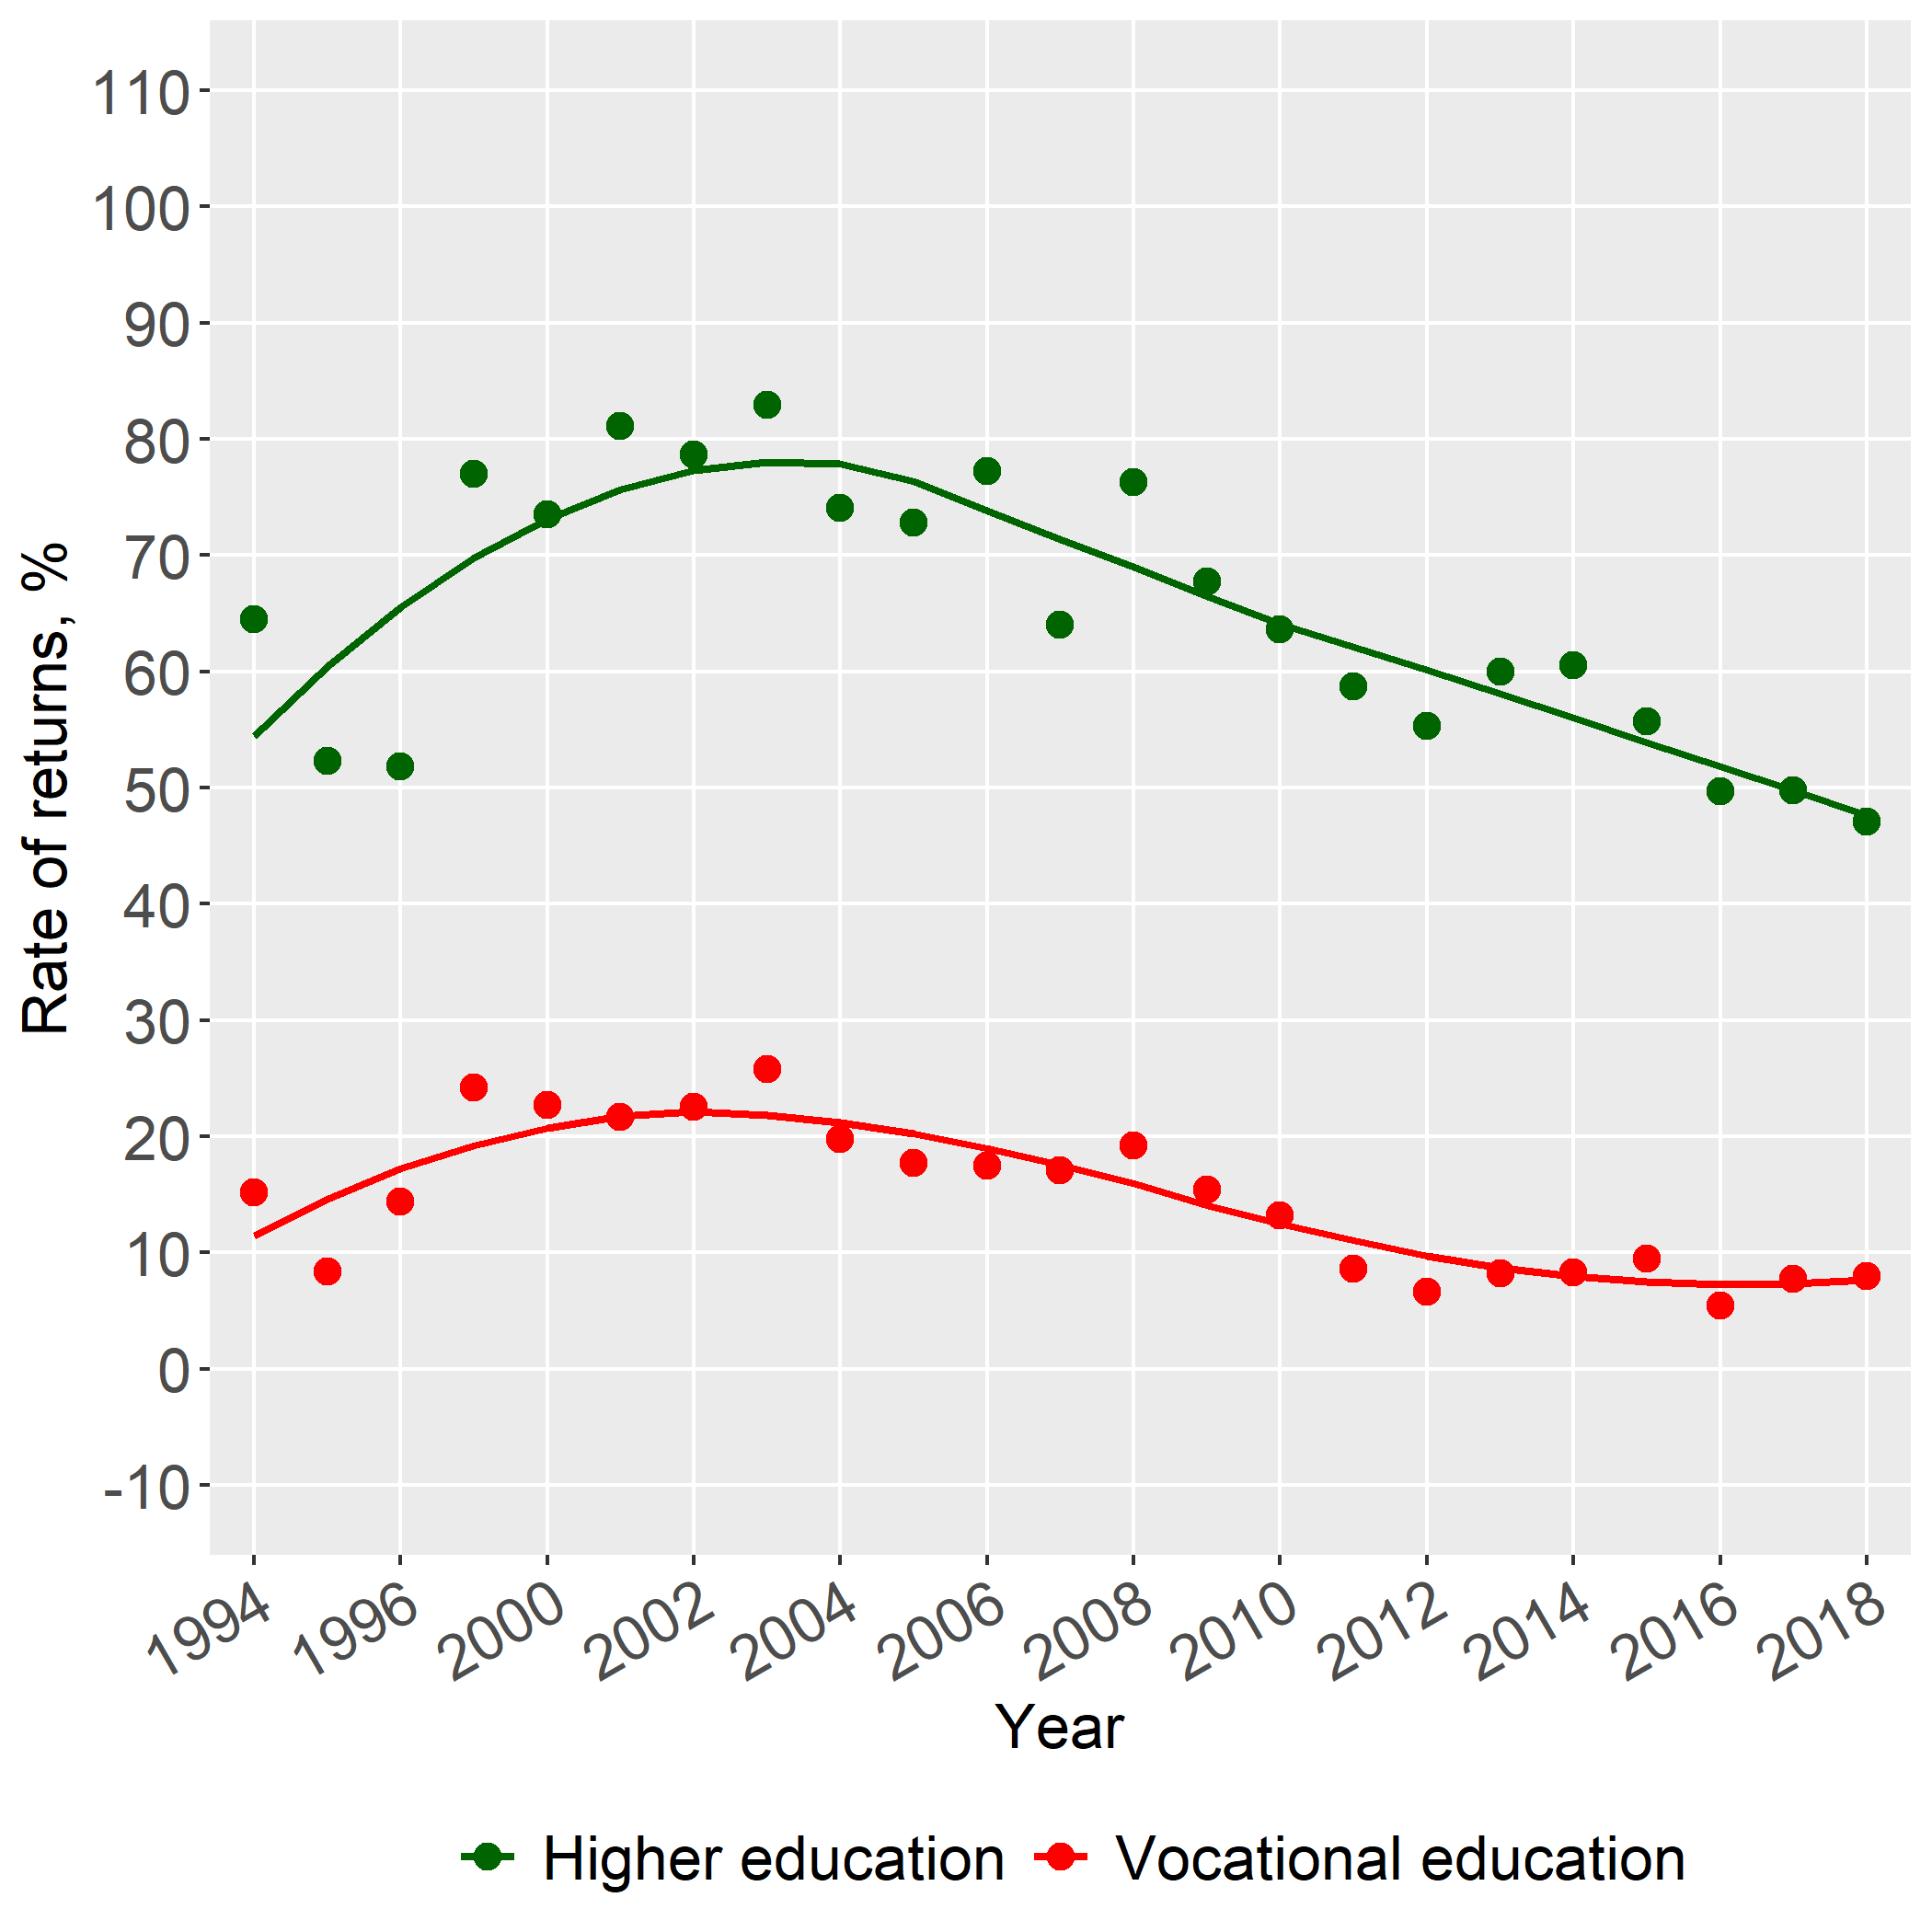
\includegraphics[width=\textwidth]{p1.png}
                 \caption{Rates of Return}
                 \label{fig:Rates}
         \end{subfigure}%
         ~ %add desired spacing between images, e. g. ~, \quad, \qquad, \hfill etc.
           %(or a blank line to force the subfigure onto a new line)
         \begin{subfigure}[b]{0.5\textwidth}
                 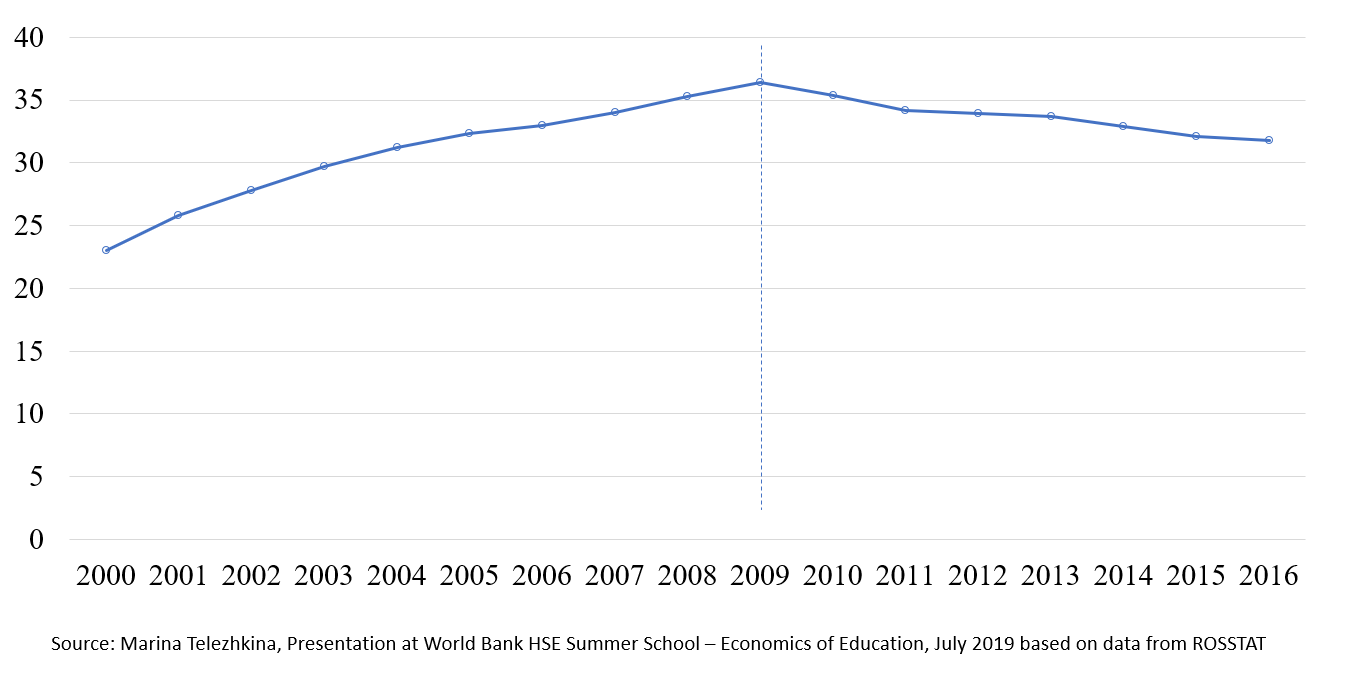
\includegraphics[width=\textwidth]{telezhkina.png}
                 \caption{Enrollment in Higher Education}
                 \label{fig:enroll}
         \end{subfigure}
     \end{figure}





When we look at the same data with information by gender, it is quite interesting that gender-based trends in Russia have a different shape across time with regard to schooling premiums. Though the percentage fluctuated slightly from year to year, there were about 55\% females in the sample compared to 45\% males. Particularly, males' payoffs to higher education (varying from 45\% to 76\%) turn out to be on a slightly decreasing slope, whereas women' returns are described by an inversely U-shaped pattern, reaching their maximum of 104\% in 2001. Within the last roughly 5 years wage premiums to higher education for women have stabilized around the level of men (~50\%).  Gender wise enrollment rates in higher education (not shown) ten years later appears to match the differences in rates of return, strengthening the hypothesis that market rates of return to education in Russia do indeed influence individual continuing school decisions. 

A similar comparative picture is observed with respect to vocational education, however, the described regularities are way less pronounced (see Figure 2): returns for males are almost flat within the time period under focus and the parabolic association for females is tangibly less concave. The overall outcome concerning payoffs to schooling isolated by gender has been confirmed in a similar fashion by past studies \parencite{cheidvasser_006._2007}, etc .


\begin{figure}[H]
  \begin{minipage}[b]{.5\linewidth}
     \centering
     \hspace*{-0.7in}
     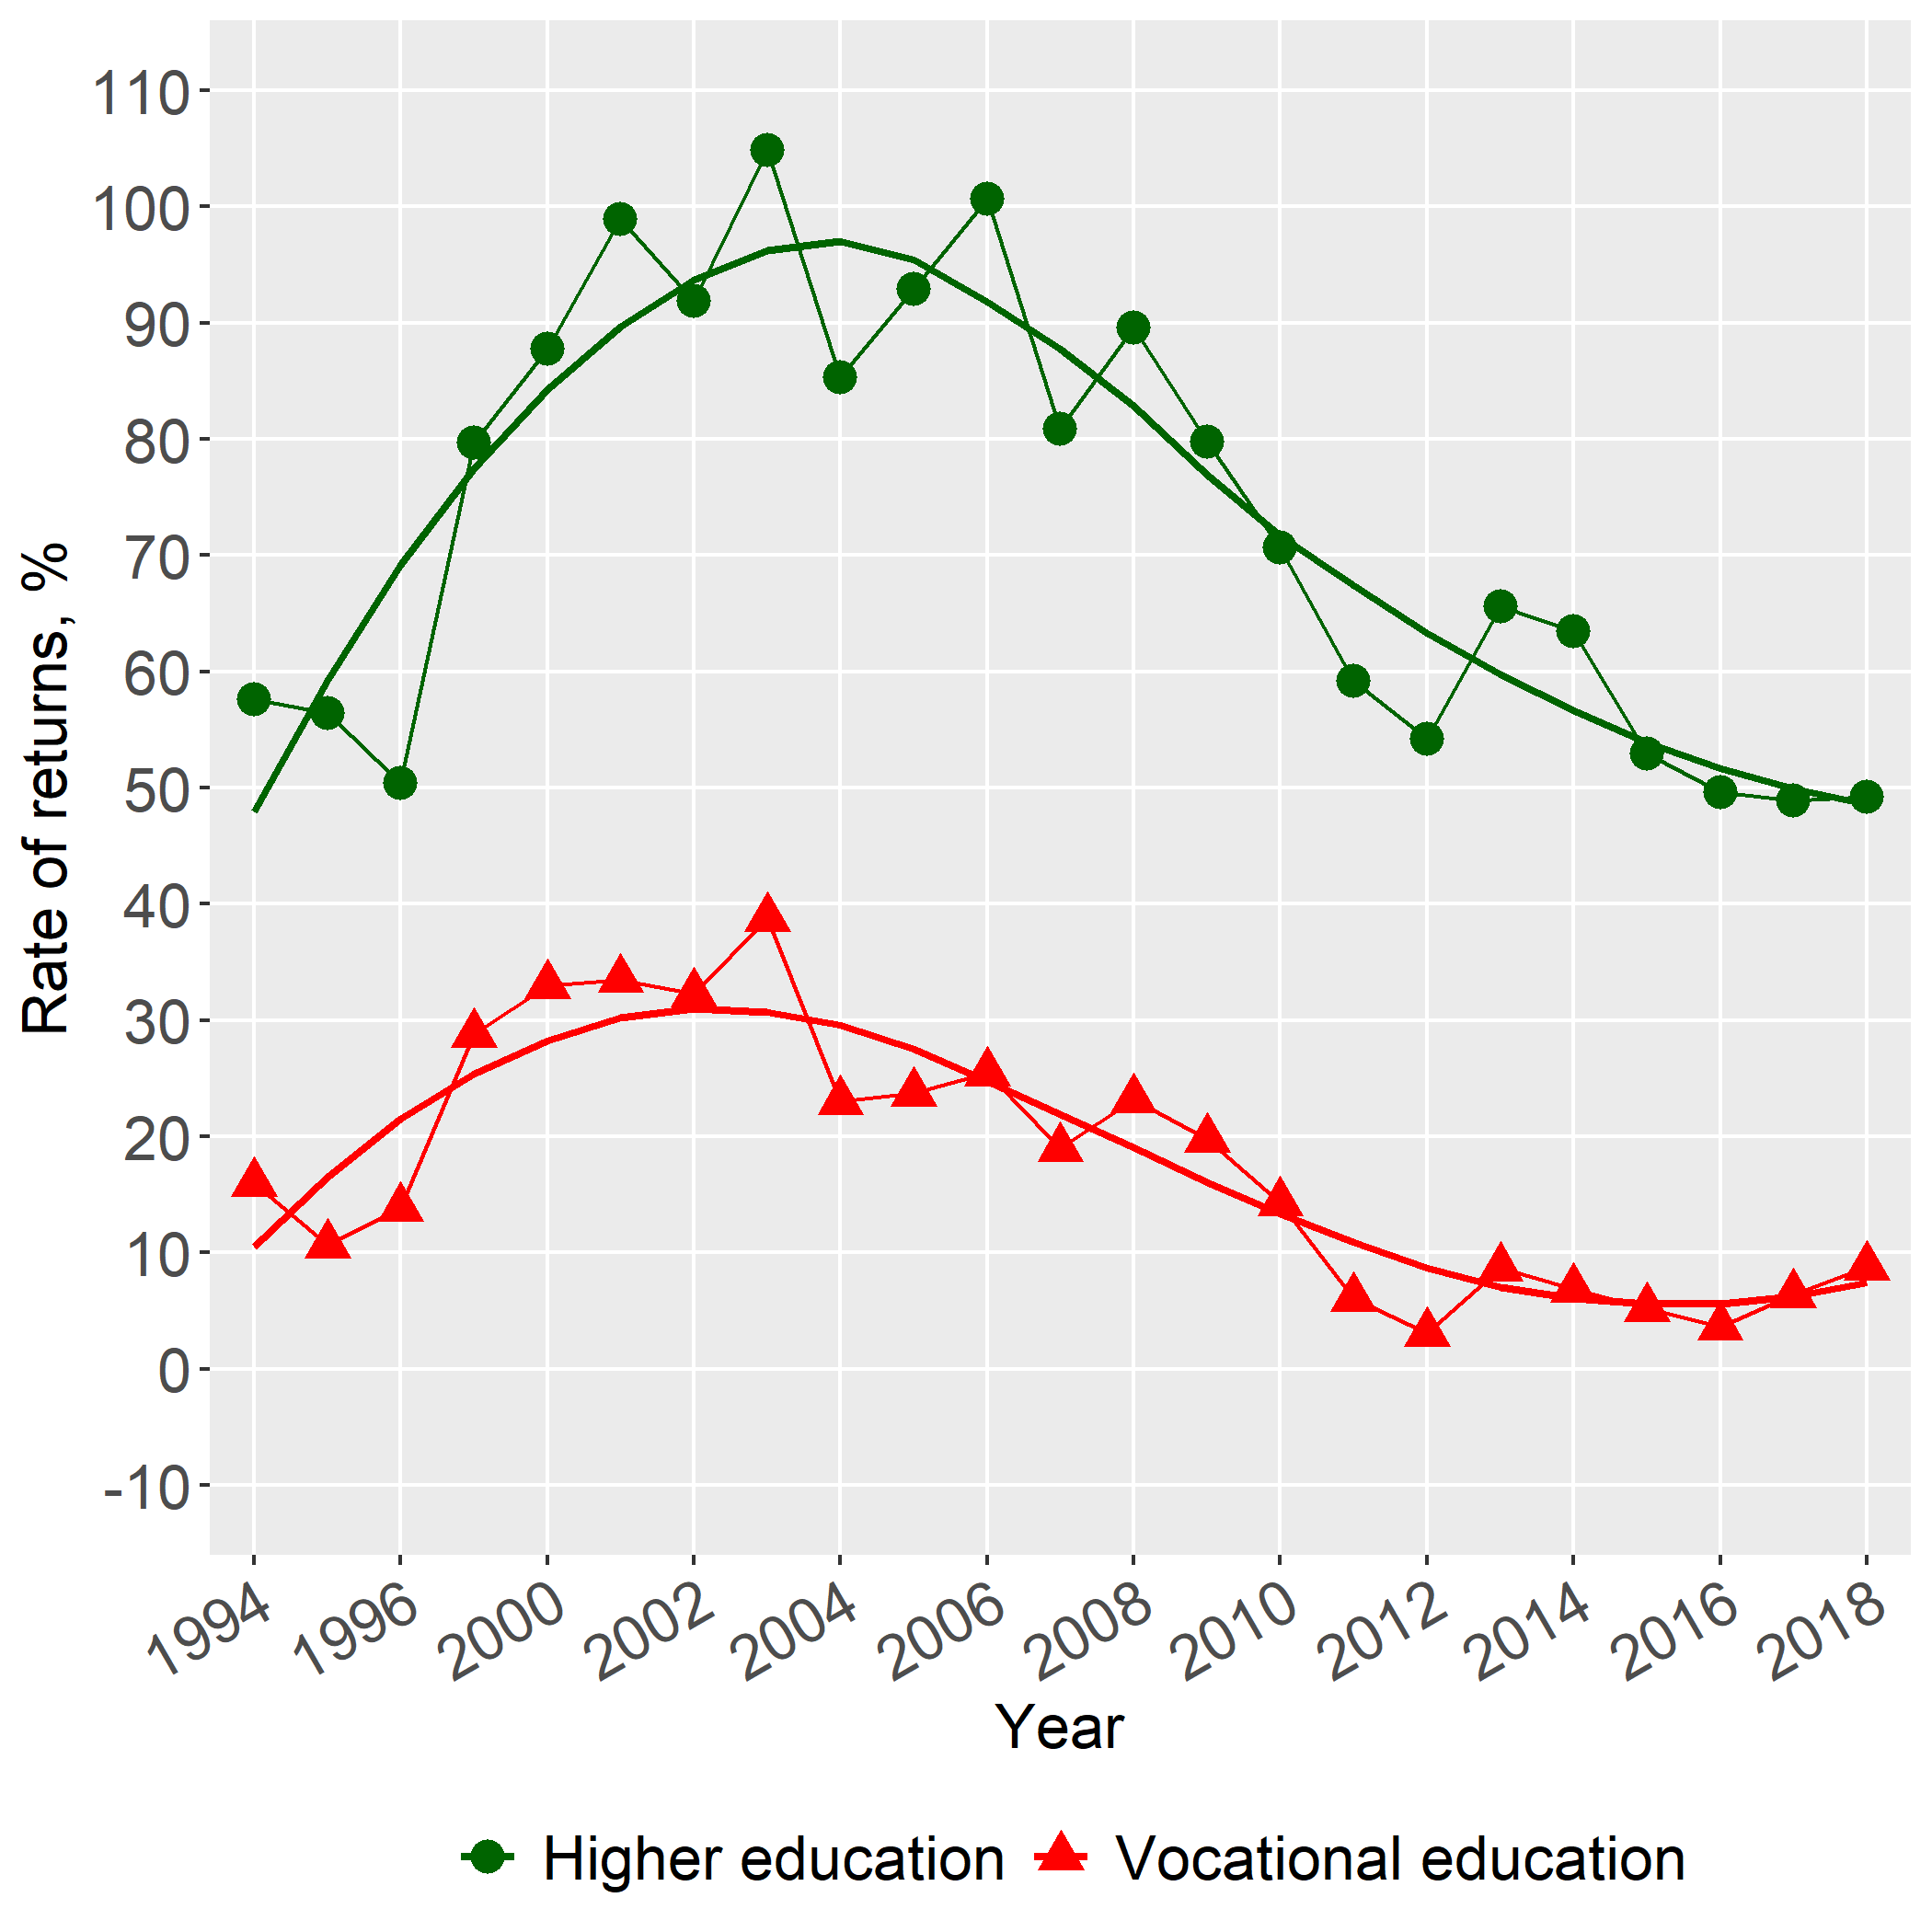
\includegraphics[width=270pt]{p2a.png}
     % plot 1
     \subcaption{Females}\label{fig:2a}
  \end{minipage}
  \hfill
  \begin{minipage}[b]{.5\linewidth}
     \centering
     \hspace*{0in}
     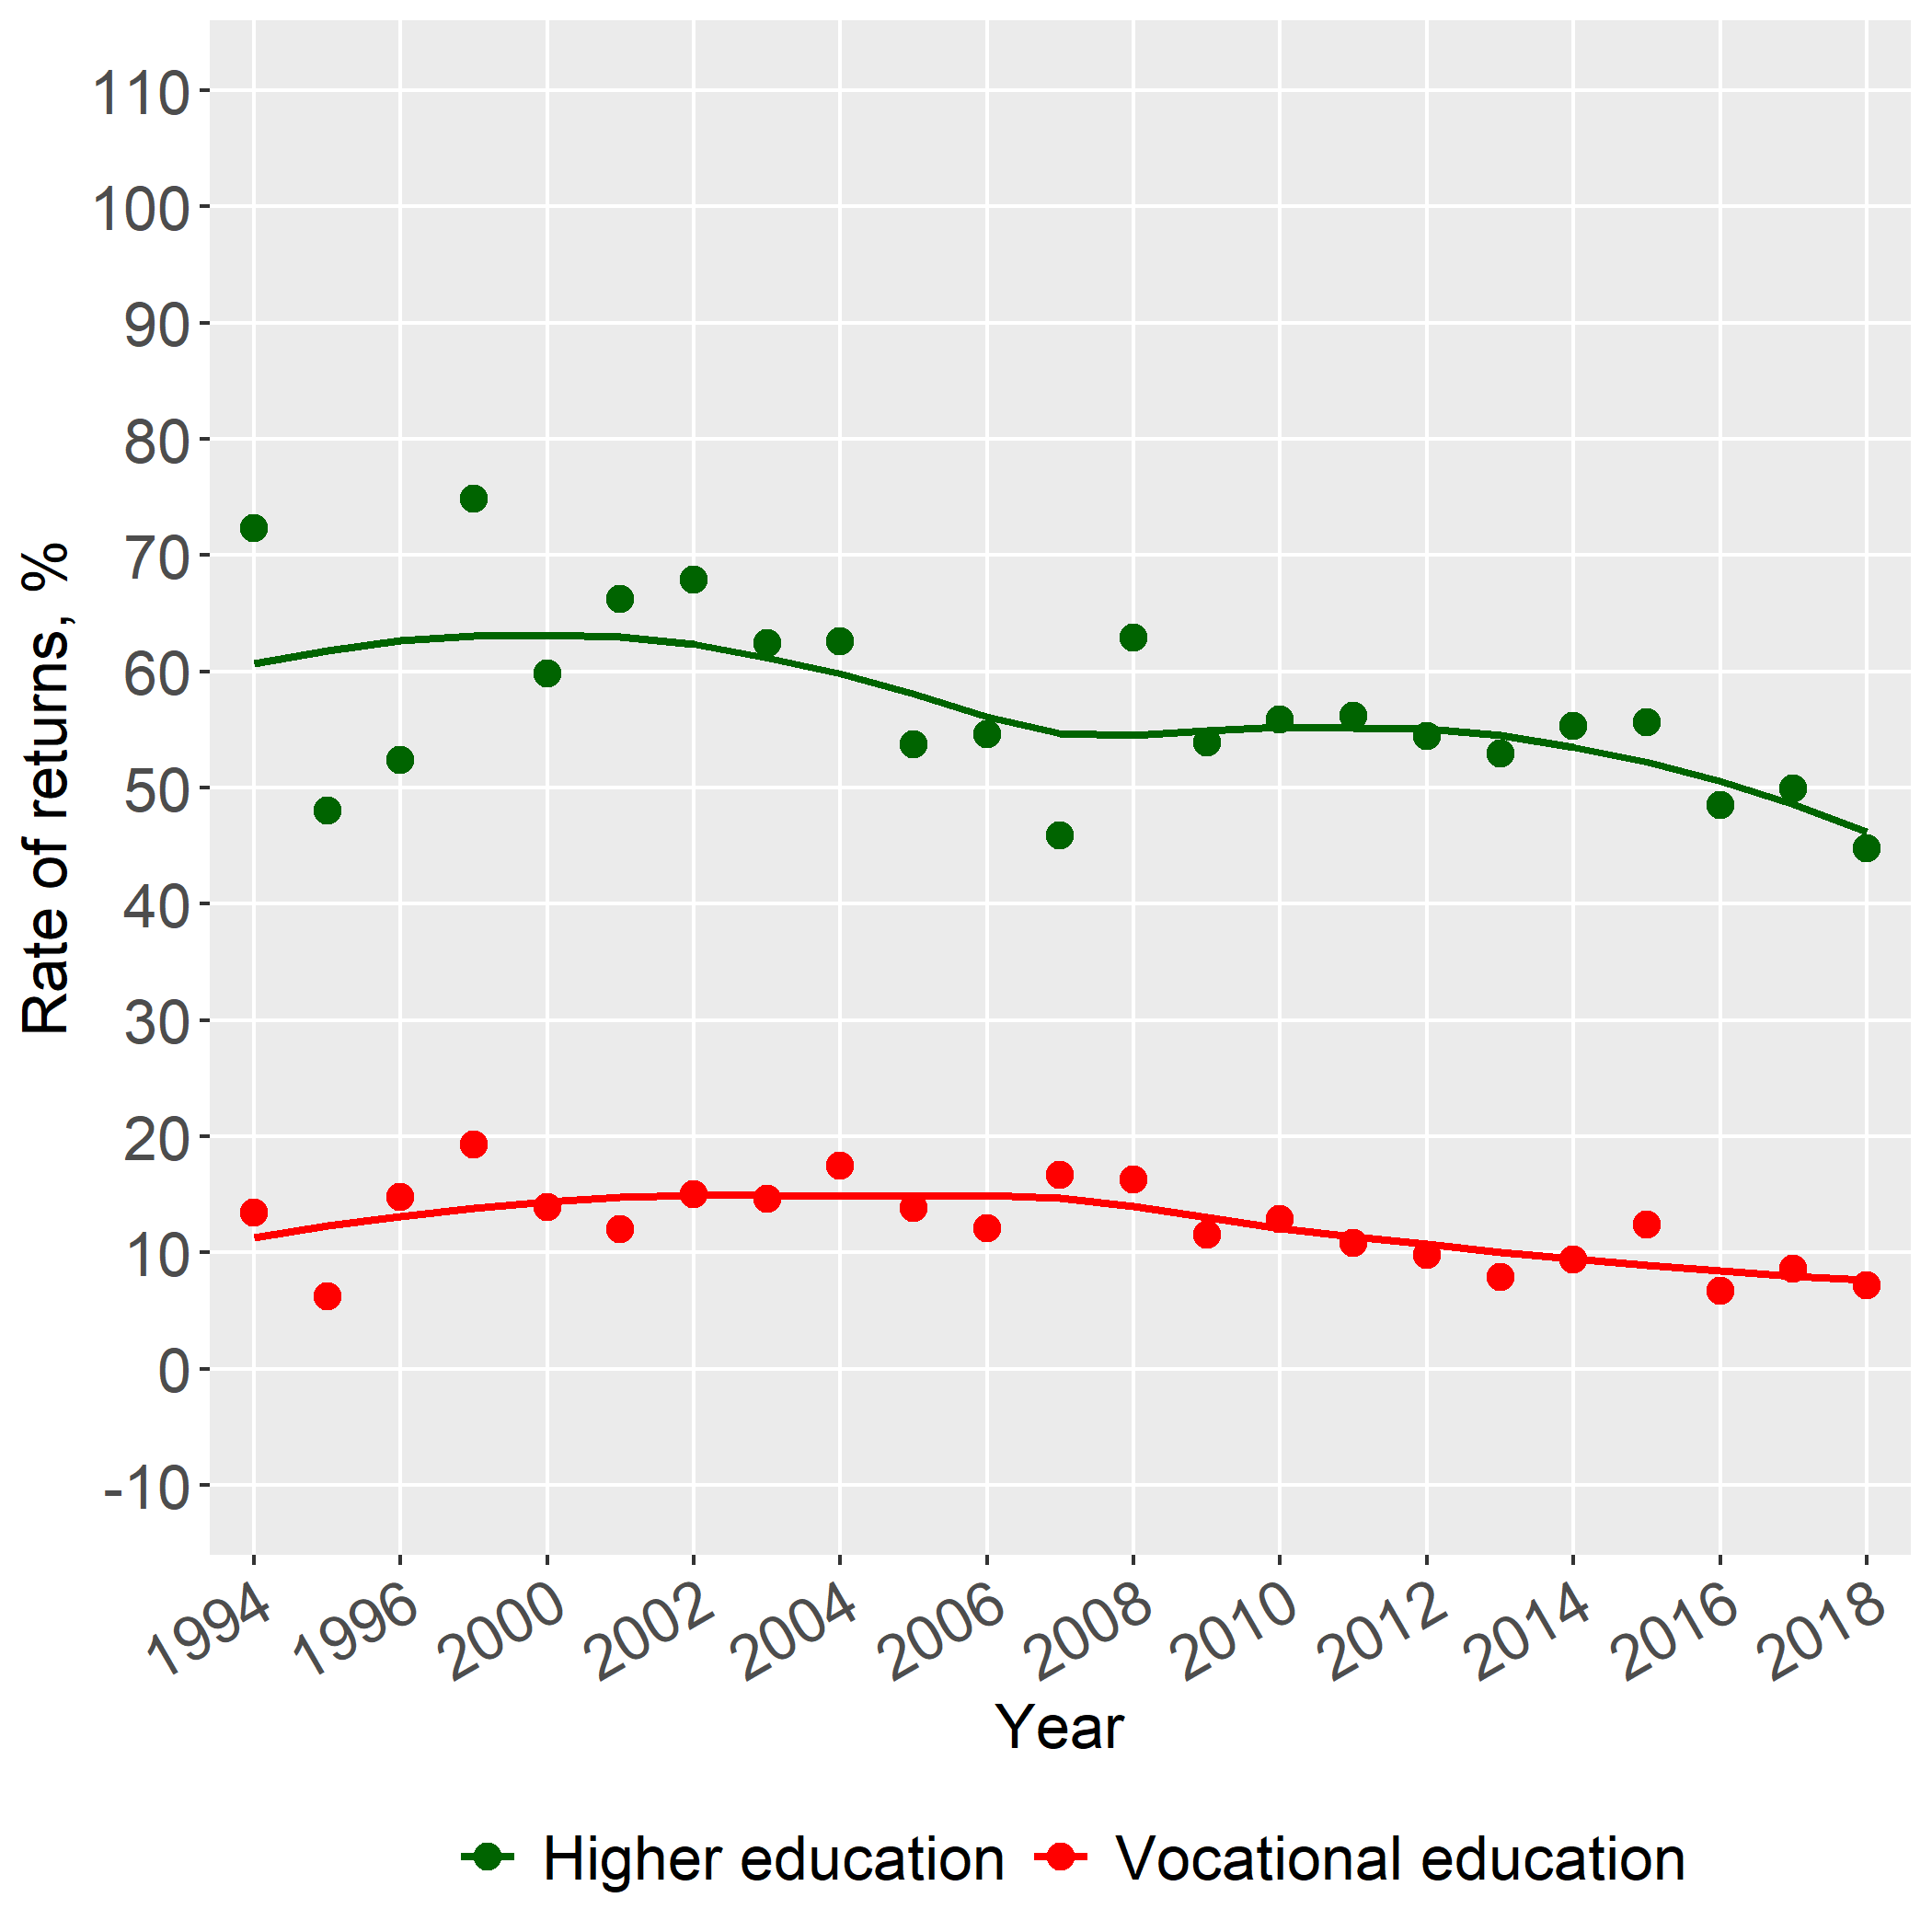
\includegraphics[width=270pt]{p2b.png}
     % plot 2
     \subcaption{Males}\label{fig:2b}
  \end{minipage}
  \caption{Rates of Returns to Higher and Vocational Education in Russia, RLMS 1994-2018}\label{fig:2}
\end{figure}

Looking at the pattern by nationality, there were approximately 15\% non Russian nationals or immigrants in the RLMS database. We find that for Russian nationals, the payoffs to higher and vocational education are characterized by a pattern almost identical to the one uncovered for the whole population. As for non-Russians, the estimates of wage advantages regarding people with university education level compared to those with only secondary level are not statistically significant in the majority of time periods investigated (except for 2002-2006 and 2008). Nevertheless, the payoffs to vocational education for those who identified themselves as non-Russians are significant and the respective time trend is loosely distinguishable from the one registered for Russians. In other words, nationality seem to affect returns to higher education, but does not play a similar part with respect to vocational education.


\begin{figure}[H]
  \begin{minipage}[b]{.5\linewidth}
     \centering
     \hspace*{-0.7in}
     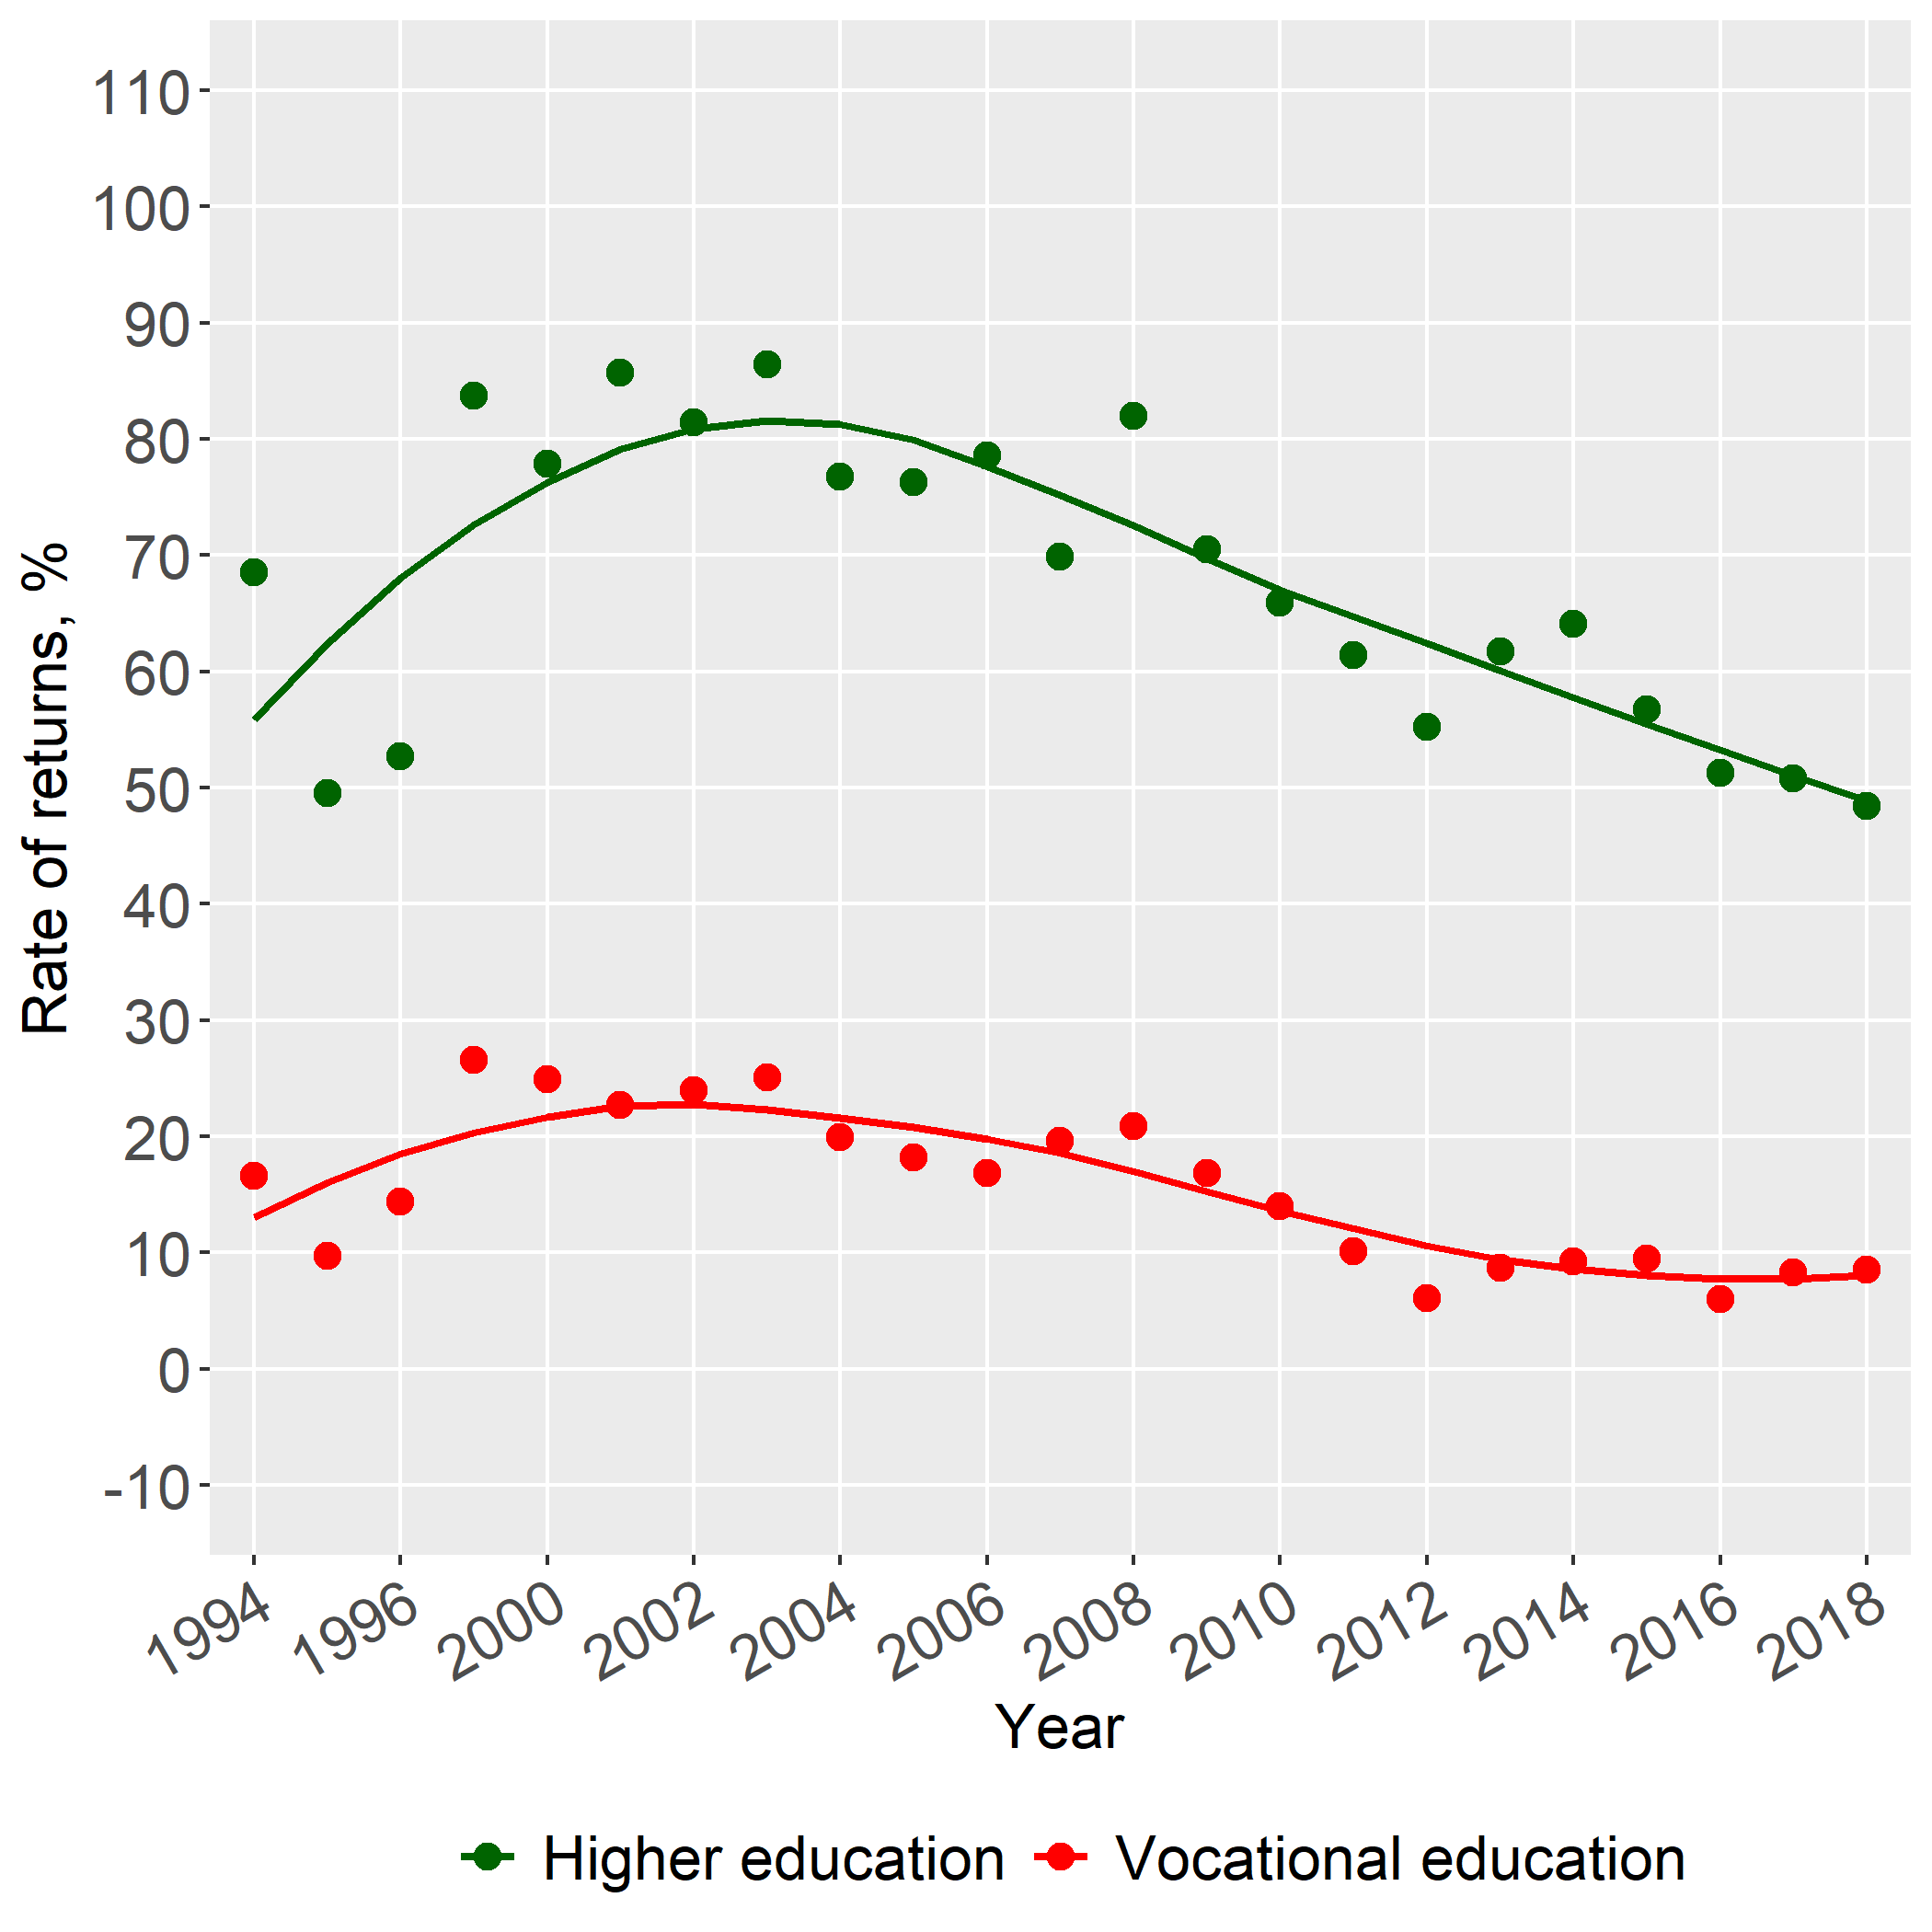
\includegraphics[width=270pt]{p3a.png}
     % plot 1
     \subcaption{Russians}\label{fig:3a}
  \end{minipage}
  \hfill
  \begin{minipage}[b]{.5\linewidth}
     \centering
     \hspace*{0in}
     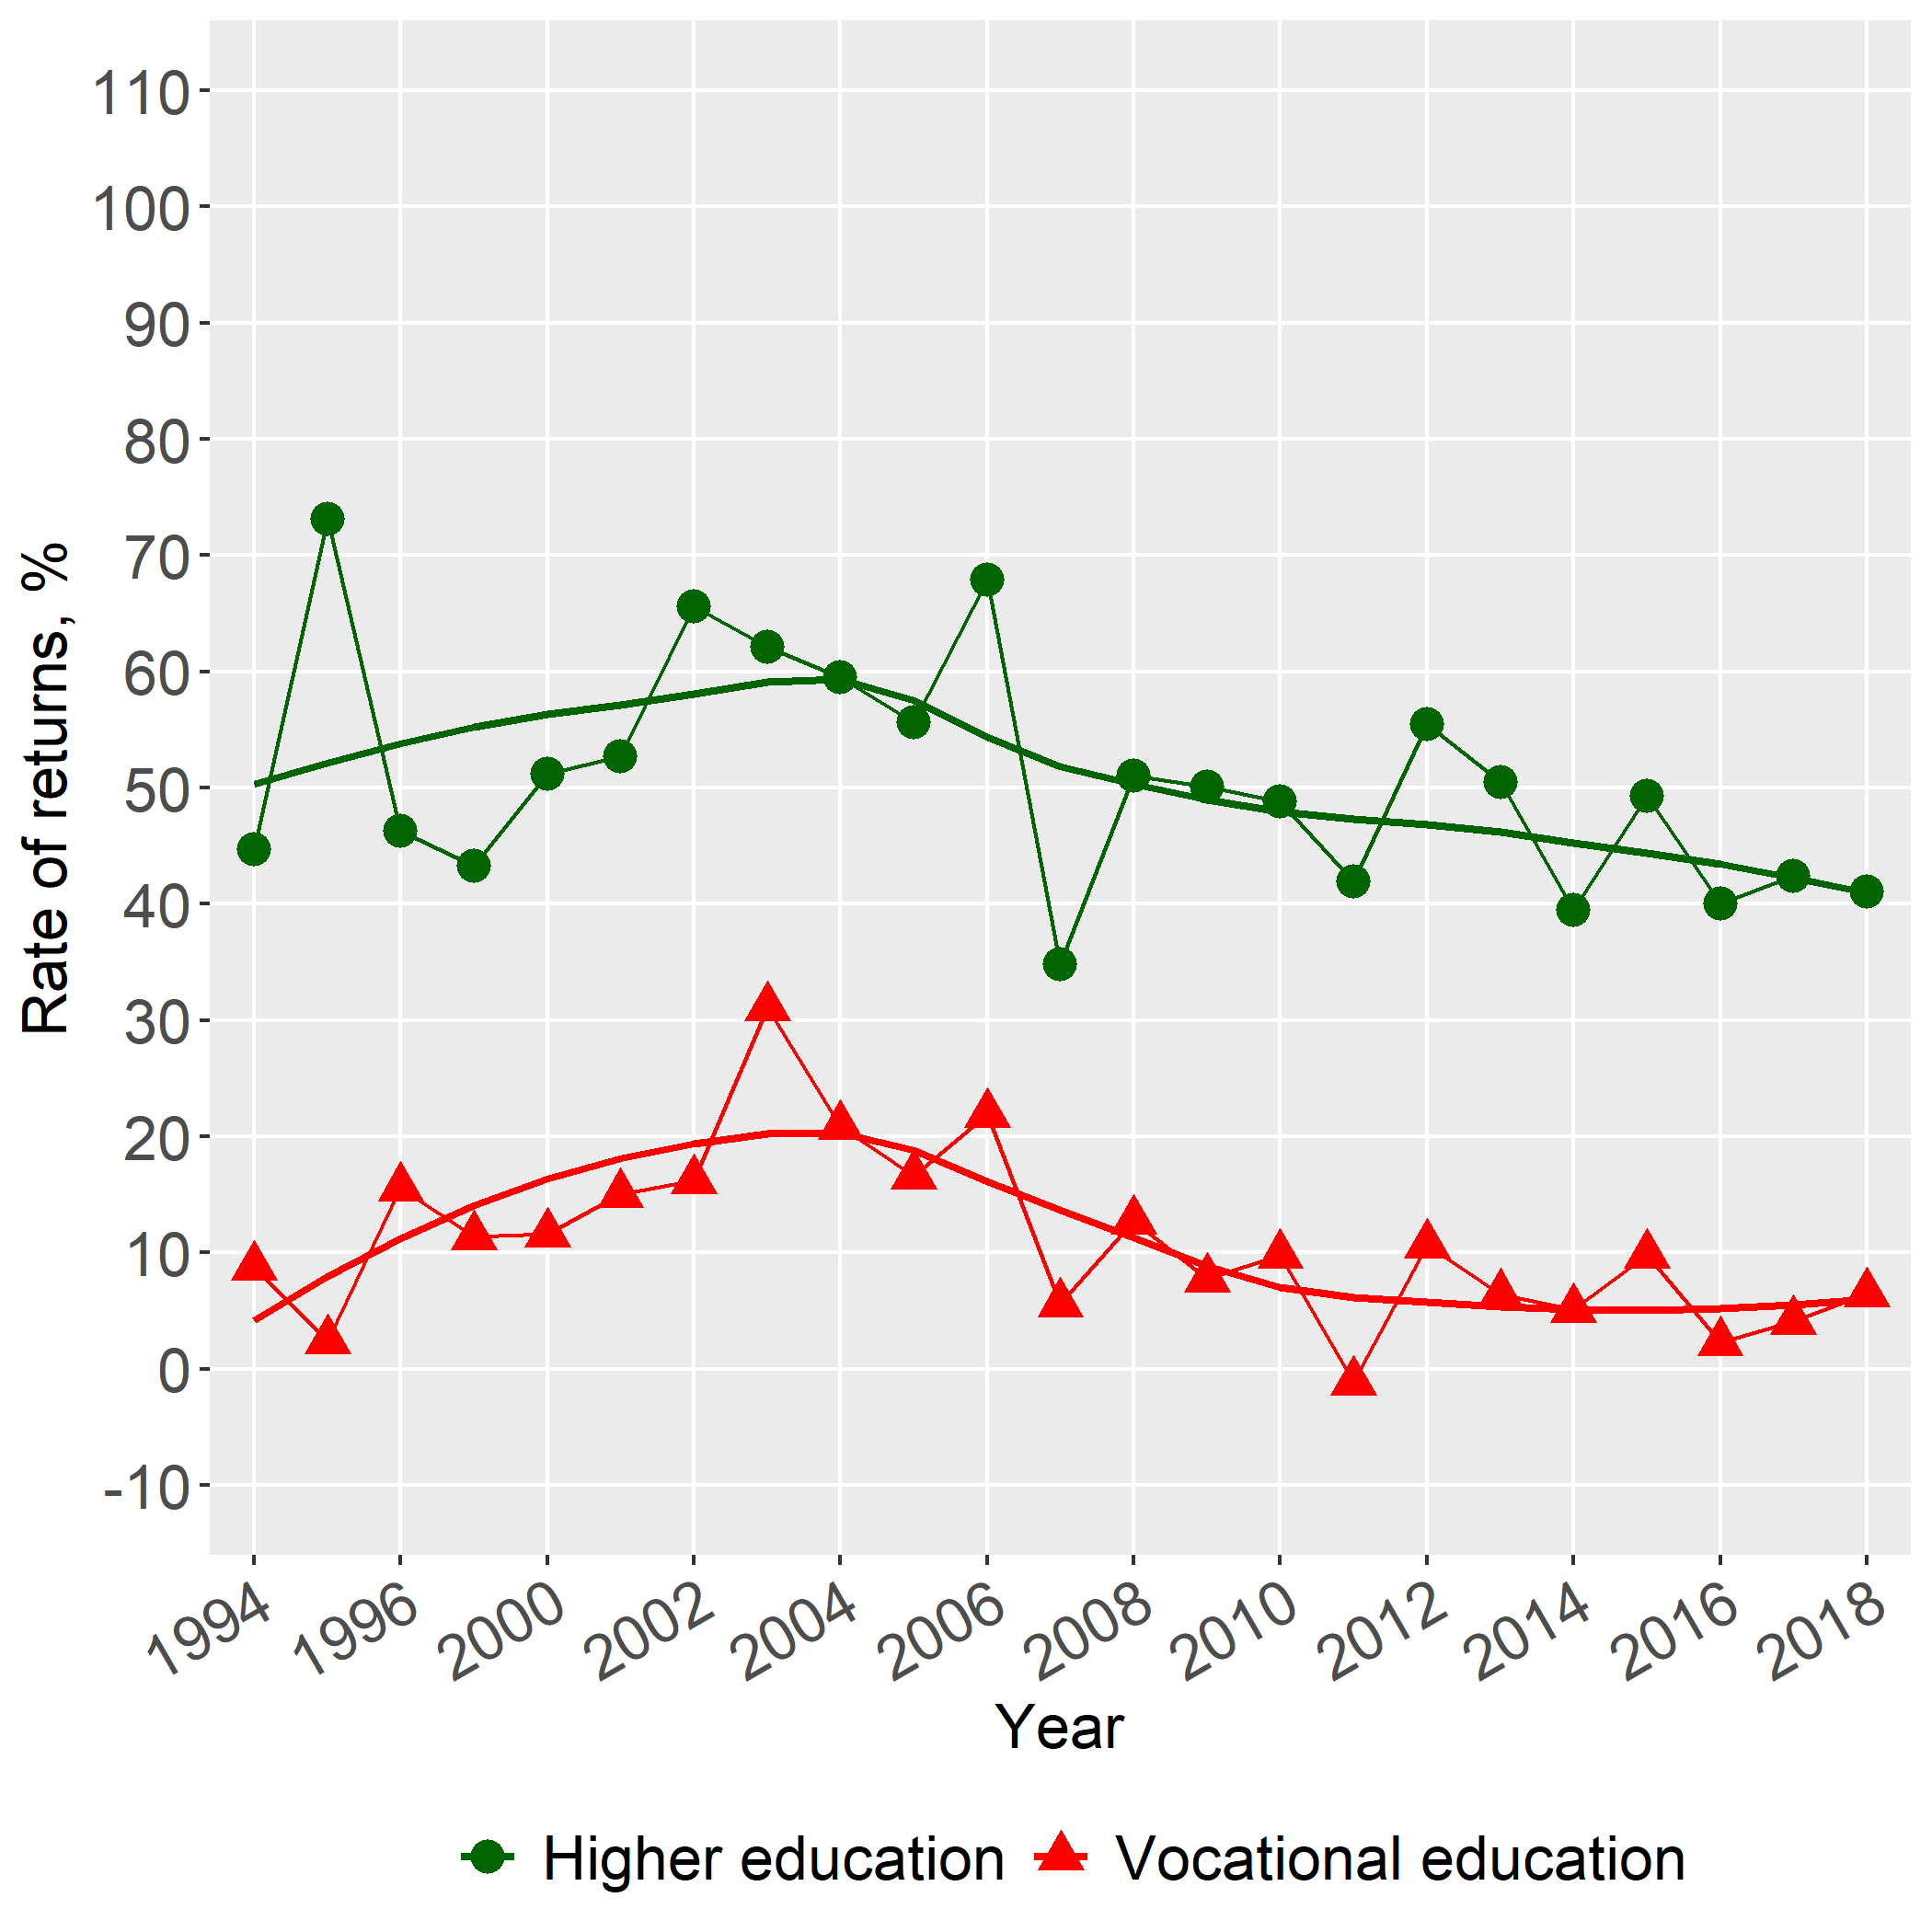
\includegraphics[width=270pt]{p3b.png}
     % plot 2
     \subcaption{Non-Russians}\label{fig:3b}
  \end{minipage}
  \caption{Rates of Returns to Higher and Vocational Education in Russia, RLMS 1994-2018}\label{fig:4}
\end{figure}

\section*{References in Russian}

 This is a Russian reference. \foreignlanguage{russian}{досвыдания}

Now I cite \parencite{carnoy_005._2012}. 

And now Russian
\selectlanguage{russian}
\parencite{blix}. 

\printbibliography

\selectlanguage{english}

\newpage
\section*{Appendix}

% Table created by stargazer v.5.2.2 by Marek Hlavac, Harvard University. E-mail: hlavac at fas.harvard.edu
% Date and time: Thu, Oct 31, 2019 - 2:41:10 PM
\begin{table}[!htbp] \centering 
  \caption{Results of Mincer Analysis, RLMS 1994} 
  \label{} 
\begin{tabular}{@{\extracolsep{5pt}}lccccc} 
\\[-1.8ex]\hline 
\hline \\[-1.8ex] 
 & Total Sample & Males & Females & Russians & Non-Russians \\ 
\\[-1.8ex] & (1) & (2) & (3) & (4) & (5)\\ 
\hline \\[-1.8ex] 
 Vocational education & 0.141$^{***}$ & 0.126$^{**}$ & 0.149$^{***}$ & 0.153$^{***}$ & 0.085 \\ 
  & (0.042) & (0.064) & (0.055) & (0.046) & (0.102) \\ 
  & & & & & \\ 
 Higher education & 0.498$^{***}$ & 0.544$^{***}$ & 0.455$^{***}$ & 0.522$^{***}$ & 0.370$^{***}$ \\ 
  & (0.047) & (0.072) & (0.062) & (0.051) & (0.121) \\ 
  & & & & & \\ 
 Experience & 0.007 & 0.008 & 0.004 & 0.001 & 0.036$^{***}$ \\ 
  & (0.005) & (0.008) & (0.007) & (0.006) & (0.013) \\ 
  & & & & & \\ 
 Experience squared & $-$0.0002 & $-$0.0004 & 0.0001 & 0.00000 & $-$0.001$^{**}$ \\ 
  & (0.0002) & (0.0003) & (0.0002) & (0.0002) & (0.0004) \\ 
  & & & & & \\ 
 Non-Russian & $-$0.004 & $-$0.056 & 0.042 &  &  \\ 
  & (0.045) & (0.069) & (0.059) &  &  \\ 
  & & & & & \\ 
 Female & $-$0.499$^{***}$ &  &  & $-$0.513$^{***}$ & $-$0.438$^{***}$ \\ 
  & (0.033) &  &  & (0.036) & (0.085) \\ 
  & & & & & \\ 
 Constant & 12.104$^{***}$ & 12.132$^{***}$ & 11.588$^{***}$ & 12.128$^{***}$ & 11.979$^{***}$ \\ 
  & (0.046) & (0.065) & (0.059) & (0.050) & (0.110) \\ 
  & & & & & \\ 
\hline \\[-1.8ex] 
Observations & 3,041 & 1,394 & 1,647 & 2,564 & 477 \\ 
R$^{2}$ & 0.103 & 0.049 & 0.041 & 0.109 & 0.083 \\ 
Adjusted R$^{2}$ & 0.101 & 0.045 & 0.038 & 0.108 & 0.073 \\ 
Residual Std. Error & 0.906 & 0.957 & 0.858 & 0.905 & 0.906 \\ 
F Statistic & 57.786$^{***}$ & 14.271$^{***}$ & 14.057$^{***}$ & 62.886$^{***}$ & 8.534$^{***}$ \\ 
\hline 
\hline \\[-1.8ex] 
\textit{Note:}  & \multicolumn{5}{r}{$^{*}$p$<$0.1; $^{**}$p$<$0.05; $^{***}$p$<$0.01} \\ 
\end{tabular} 
\end{table} 

\newpage

% Table created by stargazer v.5.2.2 by Marek Hlavac, Harvard University. E-mail: hlavac at fas.harvard.edu
% Date and time: Thu, Oct 31, 2019 - 2:41:10 PM
\begin{table}[!htbp] \centering 
  \caption{Results of Mincer Analysis, RLMS 1995} 
  \label{} 
\begin{tabular}{@{\extracolsep{5pt}}lccccc} 
\\[-1.8ex]\hline 
\hline \\[-1.8ex] 
 & Total Sample & Males & Females & Russians & Non-Russians \\ 
\\[-1.8ex] & (1) & (2) & (3) & (4) & (5)\\ 
\hline \\[-1.8ex] 
 Vocational education & 0.081$^{*}$ & 0.060 & 0.101$^{*}$ & 0.092$^{*}$ & 0.023 \\ 
  & (0.044) & (0.066) & (0.060) & (0.049) & (0.109) \\ 
  & & & & & \\ 
 Higher education & 0.421$^{***}$ & 0.392$^{***}$ & 0.447$^{***}$ & 0.402$^{***}$ & 0.549$^{***}$ \\ 
  & (0.048) & (0.072) & (0.066) & (0.053) & (0.127) \\ 
  & & & & & \\ 
 Experience & 0.002 & $-$0.002 & 0.006 & 0.002 & 0.004 \\ 
  & (0.006) & (0.009) & (0.008) & (0.006) & (0.015) \\ 
  & & & & & \\ 
 Experience squared & $-$0.0001 & $-$0.00004 & $-$0.0001 & $-$0.0001 & $-$0.00005 \\ 
  & (0.0002) & (0.0003) & (0.0002) & (0.0002) & (0.001) \\ 
  & & & & & \\ 
 Non-Russian & $-$0.041 & $-$0.061 & $-$0.021 &  &  \\ 
  & (0.047) & (0.070) & (0.064) &  &  \\ 
  & & & & & \\ 
 Female & $-$0.431$^{***}$ &  &  & $-$0.437$^{***}$ & $-$0.386$^{***}$ \\ 
  & (0.035) &  &  & (0.038) & (0.090) \\ 
  & & & & & \\ 
 Constant & 12.882$^{***}$ & 12.936$^{***}$ & 12.400$^{***}$ & 12.893$^{***}$ & 12.790$^{***}$ \\ 
  & (0.049) & (0.067) & (0.064) & (0.052) & (0.118) \\ 
  & & & & & \\ 
\hline \\[-1.8ex] 
Observations & 2,690 & 1,235 & 1,455 & 2,262 & 428 \\ 
R$^{2}$ & 0.085 & 0.032 & 0.040 & 0.082 & 0.105 \\ 
Adjusted R$^{2}$ & 0.083 & 0.028 & 0.037 & 0.080 & 0.094 \\ 
Residual Std. Error & 0.897 & 0.923 & 0.875 & 0.891 & 0.925 \\ 
F Statistic & 41.523$^{***}$ & 8.181$^{***}$ & 12.128$^{***}$ & 40.396$^{***}$ & 9.873$^{***}$ \\ 
\hline 
\hline \\[-1.8ex] 
\textit{Note:}  & \multicolumn{5}{r}{$^{*}$p$<$0.1; $^{**}$p$<$0.05; $^{***}$p$<$0.01} \\ 
\end{tabular} 
\end{table} 

\newpage

% Table created by stargazer v.5.2.2 by Marek Hlavac, Harvard University. E-mail: hlavac at fas.harvard.edu
% Date and time: Thu, Oct 31, 2019 - 2:41:10 PM
\begin{table}[!htbp] \centering 
  \caption{Results of Mincer Analysis, RLMS 1996} 
  \label{} 
\begin{tabular}{@{\extracolsep{5pt}}lccccc} 
\\[-1.8ex]\hline 
\hline \\[-1.8ex] 
 & Total Sample & Males & Females & Russians & Non-Russians \\ 
\\[-1.8ex] & (1) & (2) & (3) & (4) & (5)\\ 
\hline \\[-1.8ex] 
 Vocational education & 0.134$^{**}$ & 0.138$^{*}$ & 0.129$^{*}$ & 0.134$^{**}$ & 0.145 \\ 
  & (0.052) & (0.080) & (0.069) & (0.058) & (0.118) \\ 
  & & & & & \\ 
 Higher education & 0.417$^{***}$ & 0.421$^{***}$ & 0.408$^{***}$ & 0.423$^{***}$ & 0.381$^{***}$ \\ 
  & (0.056) & (0.086) & (0.074) & (0.062) & (0.133) \\ 
  & & & & & \\ 
 Experience & 0.008 & 0.008 & 0.007 & 0.007 & 0.019 \\ 
  & (0.006) & (0.010) & (0.008) & (0.007) & (0.018) \\ 
  & & & & & \\ 
 Experience squared & $-$0.0004$^{*}$ & $-$0.001$^{*}$ & $-$0.0002 & $-$0.0003 & $-$0.001 \\ 
  & (0.0002) & (0.0003) & (0.0003) & (0.0002) & (0.001) \\ 
  & & & & & \\ 
 Non-Russian & 0.039 & 0.043 & 0.034 &  &  \\ 
  & (0.055) & (0.083) & (0.074) &  &  \\ 
  & & & & & \\ 
 Female & $-$0.477$^{***}$ &  &  & $-$0.475$^{***}$ & $-$0.499$^{***}$ \\ 
  & (0.039) &  &  & (0.043) & (0.100) \\ 
  & & & & & \\ 
 Constant & 13.208$^{***}$ & 13.230$^{***}$ & 12.713$^{***}$ & 13.205$^{***}$ & 13.245$^{***}$ \\ 
  & (0.059) & (0.084) & (0.075) & (0.064) & (0.130) \\ 
  & & & & & \\ 
\hline \\[-1.8ex] 
Observations & 2,281 & 1,033 & 1,248 & 1,941 & 340 \\ 
R$^{2}$ & 0.087 & 0.036 & 0.029 & 0.084 & 0.104 \\ 
Adjusted R$^{2}$ & 0.084 & 0.031 & 0.025 & 0.082 & 0.091 \\ 
Residual Std. Error & 0.929 & 0.976 & 0.888 & 0.934 & 0.906 \\ 
F Statistic & 35.992$^{***}$ & 7.709$^{***}$ & 7.501$^{***}$ & 35.671$^{***}$ & 7.774$^{***}$ \\ 
\hline 
\hline \\[-1.8ex] 
\textit{Note:}  & \multicolumn{5}{r}{$^{*}$p$<$0.1; $^{**}$p$<$0.05; $^{***}$p$<$0.01} \\ 
\end{tabular} 
\end{table} 

\newpage

% Table created by stargazer v.5.2.2 by Marek Hlavac, Harvard University. E-mail: hlavac at fas.harvard.edu
% Date and time: Thu, Oct 31, 2019 - 2:41:10 PM
\begin{table}[!htbp] \centering 
  \caption{Results of Mincer Analysis, RLMS 1998} 
  \label{} 
\begin{tabular}{@{\extracolsep{5pt}}lccccc} 
\\[-1.8ex]\hline 
\hline \\[-1.8ex] 
 & Total Sample & Males & Females & Russians & Non-Russians \\ 
\\[-1.8ex] & (1) & (2) & (3) & (4) & (5)\\ 
\hline \\[-1.8ex] 
 Vocational education & 0.217$^{***}$ & 0.176$^{***}$ & 0.253$^{***}$ & 0.236$^{***}$ & 0.108 \\ 
  & (0.037) & (0.054) & (0.050) & (0.040) & (0.093) \\ 
  & & & & & \\ 
 Higher education & 0.571$^{***}$ & 0.559$^{***}$ & 0.586$^{***}$ & 0.608$^{***}$ & 0.360$^{***}$ \\ 
  & (0.041) & (0.061) & (0.054) & (0.044) & (0.106) \\ 
  & & & & & \\ 
 Experience & 0.015$^{***}$ & 0.010 & 0.020$^{***}$ & 0.014$^{***}$ & 0.022$^{*}$ \\ 
  & (0.005) & (0.007) & (0.006) & (0.005) & (0.011) \\ 
  & & & & & \\ 
 Experience squared & $-$0.0004$^{***}$ & $-$0.0004$^{*}$ & $-$0.0004$^{**}$ & $-$0.0004$^{**}$ & $-$0.001$^{*}$ \\ 
  & (0.0002) & (0.0002) & (0.0002) & (0.0002) & (0.0003) \\ 
  & & & & & \\ 
 Non-Russian & $-$0.032 & $-$0.073 & $-$0.0004 &  &  \\ 
  & (0.038) & (0.059) & (0.049) &  &  \\ 
  & & & & & \\ 
 Female & $-$0.470$^{***}$ &  &  & $-$0.483$^{***}$ & $-$0.406$^{***}$ \\ 
  & (0.028) &  &  & (0.030) & (0.071) \\ 
  & & & & & \\ 
 Constant & 6.364$^{***}$ & 6.447$^{***}$ & 5.817$^{***}$ & 6.358$^{***}$ & 6.373$^{***}$ \\ 
  & (0.043) & (0.061) & (0.057) & (0.046) & (0.107) \\ 
  & & & & & \\ 
\hline \\[-1.8ex] 
Observations & 3,101 & 1,434 & 1,667 & 2,614 & 487 \\ 
R$^{2}$ & 0.133 & 0.064 & 0.079 & 0.141 & 0.095 \\ 
Adjusted R$^{2}$ & 0.131 & 0.061 & 0.076 & 0.140 & 0.086 \\ 
Residual Std. Error & 0.768 & 0.806 & 0.733 & 0.767 & 0.770 \\ 
F Statistic & 79.074$^{***}$ & 19.512$^{***}$ & 28.374$^{***}$ & 85.755$^{***}$ & 10.119$^{***}$ \\ 
\hline 
\hline \\[-1.8ex] 
\textit{Note:}  & \multicolumn{5}{r}{$^{*}$p$<$0.1; $^{**}$p$<$0.05; $^{***}$p$<$0.01} \\ 
\end{tabular} 
\end{table} 

\newpage

% Table created by stargazer v.5.2.2 by Marek Hlavac, Harvard University. E-mail: hlavac at fas.harvard.edu
% Date and time: Thu, Oct 31, 2019 - 2:41:11 PM
\begin{table}[!htbp] \centering 
  \caption{Results of Mincer Analysis, RLMS 2000} 
  \label{} 
\begin{tabular}{@{\extracolsep{5pt}}lccccc} 
\\[-1.8ex]\hline 
\hline \\[-1.8ex] 
 & Total Sample & Males & Females & Russians & Non-Russians \\ 
\\[-1.8ex] & (1) & (2) & (3) & (4) & (5)\\ 
\hline \\[-1.8ex] 
 Vocational education & 0.205$^{***}$ & 0.131$^{**}$ & 0.285$^{***}$ & 0.222$^{***}$ & 0.110 \\ 
  & (0.039) & (0.056) & (0.053) & (0.042) & (0.101) \\ 
  & & & & & \\ 
 Higher education & 0.551$^{***}$ & 0.469$^{***}$ & 0.630$^{***}$ & 0.576$^{***}$ & 0.413$^{***}$ \\ 
  & (0.043) & (0.064) & (0.057) & (0.046) & (0.113) \\ 
  & & & & & \\ 
 Experience & 0.009$^{*}$ & 0.001 & 0.016$^{**}$ & 0.008 & 0.014 \\ 
  & (0.005) & (0.008) & (0.007) & (0.006) & (0.016) \\ 
  & & & & & \\ 
 Experience squared & $-$0.0002 & $-$0.0002 & $-$0.0002 & $-$0.0002 & $-$0.0004 \\ 
  & (0.0002) & (0.0003) & (0.0002) & (0.0002) & (0.001) \\ 
  & & & & & \\ 
 Non-Russian & $-$0.001 & $-$0.016 & 0.002 &  &  \\ 
  & (0.042) & (0.065) & (0.055) &  &  \\ 
  & & & & & \\ 
 Female & $-$0.534$^{***}$ &  &  & $-$0.536$^{***}$ & $-$0.511$^{***}$ \\ 
  & (0.030) &  &  & (0.032) & (0.081) \\ 
  & & & & & \\ 
 Constant & 7.071$^{***}$ & 7.207$^{***}$ & 6.398$^{***}$ & 7.059$^{***}$ & 7.120$^{***}$ \\ 
  & (0.046) & (0.065) & (0.062) & (0.049) & (0.123) \\ 
  & & & & & \\ 
\hline \\[-1.8ex] 
Observations & 3,213 & 1,475 & 1,738 & 2,765 & 448 \\ 
R$^{2}$ & 0.128 & 0.042 & 0.078 & 0.133 & 0.104 \\ 
Adjusted R$^{2}$ & 0.127 & 0.038 & 0.075 & 0.131 & 0.094 \\ 
Residual Std. Error & 0.830 & 0.861 & 0.799 & 0.829 & 0.835 \\ 
F Statistic & 78.748$^{***}$ & 12.777$^{***}$ & 29.233$^{***}$ & 84.557$^{***}$ & 10.307$^{***}$ \\ 
\hline 
\hline \\[-1.8ex] 
\textit{Note:}  & \multicolumn{5}{r}{$^{*}$p$<$0.1; $^{**}$p$<$0.05; $^{***}$p$<$0.01} \\ 
\end{tabular} 
\end{table} 

\newpage

% Table created by stargazer v.5.2.2 by Marek Hlavac, Harvard University. E-mail: hlavac at fas.harvard.edu
% Date and time: Thu, Oct 31, 2019 - 2:41:11 PM
\begin{table}[!htbp] \centering 
  \caption{Results of Mincer Analysis, RLMS 2001} 
  \label{} 
\begin{tabular}{@{\extracolsep{5pt}}lccccc} 
\\[-1.8ex]\hline 
\hline \\[-1.8ex] 
 & Total Sample & Males & Females & Russians & Non-Russians \\ 
\\[-1.8ex] & (1) & (2) & (3) & (4) & (5)\\ 
\hline \\[-1.8ex] 
 Vocational education & 0.196$^{***}$ & 0.113$^{**}$ & 0.289$^{***}$ & 0.204$^{***}$ & 0.140 \\ 
  & (0.036) & (0.052) & (0.050) & (0.039) & (0.101) \\ 
  & & & & & \\ 
 Higher education & 0.594$^{***}$ & 0.508$^{***}$ & 0.688$^{***}$ & 0.619$^{***}$ & 0.423$^{***}$ \\ 
  & (0.039) & (0.059) & (0.053) & (0.042) & (0.110) \\ 
  & & & & & \\ 
 Experience & 0.0002 & $-$0.0004 & $-$0.0002 & $-$0.002 & 0.017 \\ 
  & (0.005) & (0.007) & (0.006) & (0.005) & (0.015) \\ 
  & & & & & \\ 
 Experience squared & $-$0.00001 & $-$0.0001 & 0.0001 & 0.00004 & $-$0.0004 \\ 
  & (0.0001) & (0.0002) & (0.0002) & (0.0001) & (0.0005) \\ 
  & & & & & \\ 
 Non-Russian & $-$0.027 & $-$0.103$^{*}$ & 0.025 &  &  \\ 
  & (0.040) & (0.063) & (0.051) &  &  \\ 
  & & & & & \\ 
 Female & $-$0.463$^{***}$ &  &  & $-$0.478$^{***}$ & $-$0.361$^{***}$ \\ 
  & (0.027) &  &  & (0.029) & (0.081) \\ 
  & & & & & \\ 
 Constant & 7.491$^{***}$ & 7.591$^{***}$ & 6.921$^{***}$ & 7.501$^{***}$ & 7.383$^{***}$ \\ 
  & (0.041) & (0.058) & (0.057) & (0.044) & (0.116) \\ 
  & & & & & \\ 
\hline \\[-1.8ex] 
Observations & 3,604 & 1,673 & 1,931 & 3,128 & 476 \\ 
R$^{2}$ & 0.125 & 0.056 & 0.091 & 0.136 & 0.066 \\ 
Adjusted R$^{2}$ & 0.124 & 0.053 & 0.089 & 0.135 & 0.056 \\ 
Residual Std. Error & 0.813 & 0.853 & 0.774 & 0.805 & 0.858 \\ 
F Statistic & 85.935$^{***}$ & 19.738$^{***}$ & 38.626$^{***}$ & 98.701$^{***}$ & 6.661$^{***}$ \\ 
\hline 
\hline \\[-1.8ex] 
\textit{Note:}  & \multicolumn{5}{r}{$^{*}$p$<$0.1; $^{**}$p$<$0.05; $^{***}$p$<$0.01} \\ 
\end{tabular} 
\end{table} 

\newpage

% Table created by stargazer v.5.2.2 by Marek Hlavac, Harvard University. E-mail: hlavac at fas.harvard.edu
% Date and time: Thu, Oct 31, 2019 - 2:41:11 PM
\begin{table}[!htbp] \centering 
  \caption{Results of Mincer Analysis, RLMS 2002} 
  \label{} 
\begin{tabular}{@{\extracolsep{5pt}}lccccc} 
\\[-1.8ex]\hline 
\hline \\[-1.8ex] 
 & Total Sample & Males & Females & Russians & Non-Russians \\ 
\\[-1.8ex] & (1) & (2) & (3) & (4) & (5)\\ 
\hline \\[-1.8ex] 
 Vocational education & 0.203$^{***}$ & 0.140$^{***}$ & 0.280$^{***}$ & 0.215$^{***}$ & 0.150$^{*}$ \\ 
  & (0.033) & (0.047) & (0.046) & (0.036) & (0.082) \\ 
  & & & & & \\ 
 Higher education & 0.581$^{***}$ & 0.518$^{***}$ & 0.652$^{***}$ & 0.595$^{***}$ & 0.504$^{***}$ \\ 
  & (0.035) & (0.052) & (0.049) & (0.039) & (0.092) \\ 
  & & & & & \\ 
 Experience & 0.008$^{*}$ & 0.001 & 0.013$^{**}$ & 0.006 & 0.019 \\ 
  & (0.004) & (0.007) & (0.006) & (0.005) & (0.013) \\ 
  & & & & & \\ 
 Experience squared & $-$0.0001 & $-$0.0001 & $-$0.0002 & $-$0.0001 & $-$0.0004 \\ 
  & (0.0001) & (0.0002) & (0.0002) & (0.0001) & (0.0004) \\ 
  & & & & & \\ 
 Non-Russian & 0.069$^{*}$ & 0.066 & 0.062 &  &  \\ 
  & (0.035) & (0.055) & (0.046) &  &  \\ 
  & & & & & \\ 
 Female & $-$0.444$^{***}$ &  &  & $-$0.441$^{***}$ & $-$0.459$^{***}$ \\ 
  & (0.025) &  &  & (0.026) & (0.068) \\ 
  & & & & & \\ 
 Constant & 7.755$^{***}$ & 7.863$^{***}$ & 7.193$^{***}$ & 7.753$^{***}$ & 7.815$^{***}$ \\ 
  & (0.038) & (0.053) & (0.052) & (0.041) & (0.097) \\ 
  & & & & & \\ 
\hline \\[-1.8ex] 
Observations & 3,803 & 1,748 & 2,055 & 3,286 & 517 \\ 
R$^{2}$ & 0.133 & 0.062 & 0.098 & 0.134 & 0.125 \\ 
Adjusted R$^{2}$ & 0.131 & 0.059 & 0.096 & 0.133 & 0.116 \\ 
Residual Std. Error & 0.748 & 0.774 & 0.722 & 0.748 & 0.749 \\ 
F Statistic & 96.883$^{***}$ & 22.835$^{***}$ & 44.584$^{***}$ & 101.827$^{***}$ & 14.558$^{***}$ \\ 
\hline 
\hline \\[-1.8ex] 
\textit{Note:}  & \multicolumn{5}{r}{$^{*}$p$<$0.1; $^{**}$p$<$0.05; $^{***}$p$<$0.01} \\ 
\end{tabular} 
\end{table} 

\newpage

% Table created by stargazer v.5.2.2 by Marek Hlavac, Harvard University. E-mail: hlavac at fas.harvard.edu
% Date and time: Thu, Oct 31, 2019 - 2:41:11 PM
\begin{table}[!htbp] \centering 
  \caption{Results of Mincer Analysis, RLMS 2003} 
  \label{} 
\begin{tabular}{@{\extracolsep{5pt}}lccccc} 
\\[-1.8ex]\hline 
\hline \\[-1.8ex] 
 & Total Sample & Males & Females & Russians & Non-Russians \\ 
\\[-1.8ex] & (1) & (2) & (3) & (4) & (5)\\ 
\hline \\[-1.8ex] 
 Vocational education & 0.229$^{***}$ & 0.136$^{***}$ & 0.328$^{***}$ & 0.224$^{***}$ & 0.271$^{***}$ \\ 
  & (0.033) & (0.046) & (0.046) & (0.035) & (0.083) \\ 
  & & & & & \\ 
 Higher education & 0.604$^{***}$ & 0.485$^{***}$ & 0.717$^{***}$ & 0.623$^{***}$ & 0.483$^{***}$ \\ 
  & (0.035) & (0.052) & (0.048) & (0.038) & (0.090) \\ 
  & & & & & \\ 
 Experience & 0.008$^{**}$ & 0.008 & 0.009$^{*}$ & 0.009$^{**}$ & 0.006 \\ 
  & (0.004) & (0.007) & (0.006) & (0.005) & (0.012) \\ 
  & & & & & \\ 
 Experience squared & $-$0.0002 & $-$0.0004$^{*}$ & $-$0.0001 & $-$0.0002 & $-$0.0002 \\ 
  & (0.0001) & (0.0002) & (0.0002) & (0.0001) & (0.0004) \\ 
  & & & & & \\ 
 Non-Russian & 0.066$^{*}$ & 0.049 & 0.075 &  &  \\ 
  & (0.035) & (0.053) & (0.047) &  &  \\ 
  & & & & & \\ 
 Female & $-$0.491$^{***}$ &  &  & $-$0.495$^{***}$ & $-$0.468$^{***}$ \\ 
  & (0.024) &  &  & (0.026) & (0.066) \\ 
  & & & & & \\ 
 Constant & 7.970$^{***}$ & 8.086$^{***}$ & 7.359$^{***}$ & 7.963$^{***}$ & 8.078$^{***}$ \\ 
  & (0.038) & (0.054) & (0.052) & (0.041) & (0.099) \\ 
  & & & & & \\ 
\hline \\[-1.8ex] 
Observations & 3,857 & 1,765 & 2,092 & 3,335 & 522 \\ 
R$^{2}$ & 0.151 & 0.060 & 0.110 & 0.154 & 0.137 \\ 
Adjusted R$^{2}$ & 0.150 & 0.057 & 0.108 & 0.153 & 0.129 \\ 
Residual Std. Error & 0.747 & 0.761 & 0.731 & 0.749 & 0.731 \\ 
F Statistic & 114.015$^{***}$ & 22.345$^{***}$ & 51.464$^{***}$ & 121.088$^{***}$ & 16.378$^{***}$ \\ 
\hline 
\hline \\[-1.8ex] 
\textit{Note:}  & \multicolumn{5}{r}{$^{*}$p$<$0.1; $^{**}$p$<$0.05; $^{***}$p$<$0.01} \\ 
\end{tabular} 
\end{table} 

\newpage

% Table created by stargazer v.5.2.2 by Marek Hlavac, Harvard University. E-mail: hlavac at fas.harvard.edu
% Date and time: Thu, Oct 31, 2019 - 2:41:11 PM
\begin{table}[!htbp] \centering 
  \caption{Results of Mincer Analysis, RLMS 2004} 
  \label{} 
\begin{tabular}{@{\extracolsep{5pt}}lccccc} 
\\[-1.8ex]\hline 
\hline \\[-1.8ex] 
 & Total Sample & Males & Females & Russians & Non-Russians \\ 
\\[-1.8ex] & (1) & (2) & (3) & (4) & (5)\\ 
\hline \\[-1.8ex] 
 Vocational education & 0.181$^{***}$ & 0.161$^{***}$ & 0.207$^{***}$ & 0.181$^{***}$ & 0.189$^{**}$ \\ 
  & (0.031) & (0.044) & (0.044) & (0.034) & (0.080) \\ 
  & & & & & \\ 
 Higher education & 0.554$^{***}$ & 0.486$^{***}$ & 0.617$^{***}$ & 0.570$^{***}$ & 0.467$^{***}$ \\ 
  & (0.033) & (0.049) & (0.046) & (0.036) & (0.086) \\ 
  & & & & & \\ 
 Experience & 0.0001 & $-$0.006 & 0.005 & 0.001 & $-$0.009 \\ 
  & (0.004) & (0.006) & (0.005) & (0.004) & (0.011) \\ 
  & & & & & \\ 
 Experience squared & 0.00003 & 0.00002 & 0.00001 & $-$0.00002 & 0.0004 \\ 
  & (0.0001) & (0.0002) & (0.0002) & (0.0001) & (0.0003) \\ 
  & & & & & \\ 
 Non-Russian & 0.039 & 0.037 & 0.036 &  &  \\ 
  & (0.033) & (0.050) & (0.044) &  &  \\ 
  & & & & & \\ 
 Female & $-$0.497$^{***}$ &  &  & $-$0.497$^{***}$ & $-$0.505$^{***}$ \\ 
  & (0.023) &  &  & (0.025) & (0.063) \\ 
  & & & & & \\ 
 Constant & 8.294$^{***}$ & 8.380$^{***}$ & 7.708$^{***}$ & 8.284$^{***}$ & 8.393$^{***}$ \\ 
  & (0.036) & (0.050) & (0.049) & (0.039) & (0.089) \\ 
  & & & & & \\ 
\hline \\[-1.8ex] 
Observations & 3,967 & 1,824 & 2,143 & 3,439 & 528 \\ 
R$^{2}$ & 0.157 & 0.061 & 0.101 & 0.159 & 0.151 \\ 
Adjusted R$^{2}$ & 0.156 & 0.058 & 0.099 & 0.158 & 0.143 \\ 
Residual Std. Error & 0.711 & 0.730 & 0.692 & 0.712 & 0.707 \\ 
F Statistic & 123.291$^{***}$ & 23.549$^{***}$ & 48.085$^{***}$ & 129.807$^{***}$ & 18.629$^{***}$ \\ 
\hline 
\hline \\[-1.8ex] 
\textit{Note:}  & \multicolumn{5}{r}{$^{*}$p$<$0.1; $^{**}$p$<$0.05; $^{***}$p$<$0.01} \\ 
\end{tabular} 
\end{table} 

\newpage

% Table created by stargazer v.5.2.2 by Marek Hlavac, Harvard University. E-mail: hlavac at fas.harvard.edu
% Date and time: Thu, Oct 31, 2019 - 2:41:12 PM
\begin{table}[!htbp] \centering 
  \caption{Results of Mincer Analysis, RLMS 2005} 
  \label{} 
\begin{tabular}{@{\extracolsep{5pt}}lccccc} 
\\[-1.8ex]\hline 
\hline \\[-1.8ex] 
 & Total Sample & Males & Females & Russians & Non-Russians \\ 
\\[-1.8ex] & (1) & (2) & (3) & (4) & (5)\\ 
\hline \\[-1.8ex] 
 Vocational education & 0.163$^{***}$ & 0.129$^{***}$ & 0.212$^{***}$ & 0.167$^{***}$ & 0.154$^{*}$ \\ 
  & (0.031) & (0.043) & (0.044) & (0.034) & (0.079) \\ 
  & & & & & \\ 
 Higher education & 0.547$^{***}$ & 0.430$^{***}$ & 0.657$^{***}$ & 0.567$^{***}$ & 0.442$^{***}$ \\ 
  & (0.033) & (0.048) & (0.046) & (0.036) & (0.085) \\ 
  & & & & & \\ 
 Experience & $-$0.003 & $-$0.007 & 0.001 & $-$0.002 & $-$0.008 \\ 
  & (0.004) & (0.006) & (0.005) & (0.004) & (0.011) \\ 
  & & & & & \\ 
 Experience squared & 0.0001 & 0.00002 & 0.0001 & 0.0001 & 0.0002 \\ 
  & (0.0001) & (0.0002) & (0.0002) & (0.0001) & (0.0003) \\ 
  & & & & & \\ 
 Non-Russian & 0.063$^{*}$ & 0.016 & 0.109$^{**}$ &  &  \\ 
  & (0.033) & (0.049) & (0.044) &  &  \\ 
  & & & & & \\ 
 Female & $-$0.503$^{***}$ &  &  & $-$0.517$^{***}$ & $-$0.427$^{***}$ \\ 
  & (0.023) &  &  & (0.025) & (0.064) \\ 
  & & & & & \\ 
 Constant & 8.532$^{***}$ & 8.644$^{***}$ & 7.906$^{***}$ & 8.524$^{***}$ & 8.633$^{***}$ \\ 
  & (0.036) & (0.050) & (0.051) & (0.039) & (0.092) \\ 
  & & & & & \\ 
\hline \\[-1.8ex] 
Observations & 3,913 & 1,801 & 2,112 & 3,367 & 546 \\ 
R$^{2}$ & 0.162 & 0.053 & 0.120 & 0.169 & 0.124 \\ 
Adjusted R$^{2}$ & 0.160 & 0.050 & 0.118 & 0.167 & 0.116 \\ 
Residual Std. Error & 0.704 & 0.723 & 0.684 & 0.700 & 0.733 \\ 
F Statistic & 125.554$^{***}$ & 20.059$^{***}$ & 57.218$^{***}$ & 136.313$^{***}$ & 15.263$^{***}$ \\ 
\hline 
\hline \\[-1.8ex] 
\textit{Note:}  & \multicolumn{5}{r}{$^{*}$p$<$0.1; $^{**}$p$<$0.05; $^{***}$p$<$0.01} \\ 
\end{tabular} 
\end{table} 

\newpage

% Table created by stargazer v.5.2.2 by Marek Hlavac, Harvard University. E-mail: hlavac at fas.harvard.edu
% Date and time: Thu, Oct 31, 2019 - 2:41:12 PM
\begin{table}[!htbp] \centering 
  \caption{Results of Mincer Analysis, RLMS 2006} 
  \label{} 
\begin{tabular}{@{\extracolsep{5pt}}lccccc} 
\\[-1.8ex]\hline 
\hline \\[-1.8ex] 
 & Total Sample & Males & Females & Russians & Non-Russians \\ 
\\[-1.8ex] & (1) & (2) & (3) & (4) & (5)\\ 
\hline \\[-1.8ex] 
 Vocational education & 0.161$^{***}$ & 0.114$^{***}$ & 0.227$^{***}$ & 0.155$^{***}$ & 0.198$^{***}$ \\ 
  & (0.027) & (0.038) & (0.039) & (0.029) & (0.069) \\ 
  & & & & & \\ 
 Higher education & 0.572$^{***}$ & 0.436$^{***}$ & 0.696$^{***}$ & 0.580$^{***}$ & 0.518$^{***}$ \\ 
  & (0.029) & (0.043) & (0.041) & (0.032) & (0.075) \\ 
  & & & & & \\ 
 Experience & $-$0.003 & 0.002 & $-$0.006 & $-$0.002 & $-$0.005 \\ 
  & (0.003) & (0.005) & (0.004) & (0.004) & (0.009) \\ 
  & & & & & \\ 
 Experience squared & 0.00003 & $-$0.0002 & 0.0002 & 0.00002 & 0.0001 \\ 
  & (0.0001) & (0.0002) & (0.0001) & (0.0001) & (0.0003) \\ 
  & & & & & \\ 
 Non-Russian & 0.092$^{***}$ & 0.066 & 0.117$^{***}$ &  &  \\ 
  & (0.029) & (0.044) & (0.039) &  &  \\ 
  & & & & & \\ 
 Female & $-$0.456$^{***}$ &  &  & $-$0.463$^{***}$ & $-$0.411$^{***}$ \\ 
  & (0.020) &  &  & (0.022) & (0.054) \\ 
  & & & & & \\ 
 Constant & 8.733$^{***}$ & 8.791$^{***}$ & 8.200$^{***}$ & 8.735$^{***}$ & 8.819$^{***}$ \\ 
  & (0.031) & (0.042) & (0.043) & (0.033) & (0.078) \\ 
  & & & & & \\ 
\hline \\[-1.8ex] 
Observations & 4,804 & 2,172 & 2,632 & 4,179 & 625 \\ 
R$^{2}$ & 0.163 & 0.059 & 0.133 & 0.164 & 0.151 \\ 
Adjusted R$^{2}$ & 0.162 & 0.057 & 0.131 & 0.163 & 0.144 \\ 
Residual Std. Error & 0.681 & 0.694 & 0.667 & 0.684 & 0.659 \\ 
F Statistic & 156.012$^{***}$ & 27.246$^{***}$ & 80.635$^{***}$ & 163.550$^{***}$ & 22.059$^{***}$ \\ 
\hline 
\hline \\[-1.8ex] 
\textit{Note:}  & \multicolumn{5}{r}{$^{*}$p$<$0.1; $^{**}$p$<$0.05; $^{***}$p$<$0.01} \\ 
\end{tabular} 
\end{table} 

\newpage

% Table created by stargazer v.5.2.2 by Marek Hlavac, Harvard University. E-mail: hlavac at fas.harvard.edu
% Date and time: Thu, Oct 31, 2019 - 2:41:12 PM
\begin{table}[!htbp] \centering 
  \caption{Results of Mincer Analysis, RLMS 2007} 
  \label{} 
\begin{tabular}{@{\extracolsep{5pt}}lccccc} 
\\[-1.8ex]\hline 
\hline \\[-1.8ex] 
 & Total Sample & Males & Females & Russians & Non-Russians \\ 
\\[-1.8ex] & (1) & (2) & (3) & (4) & (5)\\ 
\hline \\[-1.8ex] 
 Vocational education & 0.158$^{***}$ & 0.155$^{***}$ & 0.174$^{***}$ & 0.179$^{***}$ & 0.054 \\ 
  & (0.026) & (0.035) & (0.037) & (0.028) & (0.066) \\ 
  & & & & & \\ 
 Higher education & 0.495$^{***}$ & 0.378$^{***}$ & 0.593$^{***}$ & 0.530$^{***}$ & 0.298$^{***}$ \\ 
  & (0.028) & (0.039) & (0.039) & (0.030) & (0.072) \\ 
  & & & & & \\ 
 Experience & $-$0.001 & 0.002 & $-$0.003 & $-$0.003 & 0.011 \\ 
  & (0.003) & (0.005) & (0.004) & (0.003) & (0.009) \\ 
  & & & & & \\ 
 Experience squared & $-$0.00005 & $-$0.0002$^{*}$ & 0.0001 & 0.00000 & $-$0.0004 \\ 
  & (0.0001) & (0.0001) & (0.0001) & (0.0001) & (0.0003) \\ 
  & & & & & \\ 
 Non-Russian & 0.045 & $-$0.019 & 0.110$^{***}$ &  &  \\ 
  & (0.028) & (0.041) & (0.038) &  &  \\ 
  & & & & & \\ 
 Female & $-$0.429$^{***}$ &  &  & $-$0.447$^{***}$ & $-$0.318$^{***}$ \\ 
  & (0.019) &  &  & (0.020) & (0.053) \\ 
  & & & & & \\ 
 Constant & 8.955$^{***}$ & 9.000$^{***}$ & 8.476$^{***}$ & 8.953$^{***}$ & 8.996$^{***}$ \\ 
  & (0.029) & (0.040) & (0.040) & (0.031) & (0.076) \\ 
  & & & & & \\ 
\hline \\[-1.8ex] 
Observations & 4,726 & 2,153 & 2,573 & 4,136 & 590 \\ 
R$^{2}$ & 0.152 & 0.050 & 0.113 & 0.161 & 0.097 \\ 
Adjusted R$^{2}$ & 0.150 & 0.048 & 0.111 & 0.160 & 0.089 \\ 
Residual Std. Error & 0.640 & 0.641 & 0.636 & 0.641 & 0.631 \\ 
F Statistic & 140.495$^{***}$ & 22.629$^{***}$ & 65.411$^{***}$ & 158.888$^{***}$ & 12.539$^{***}$ \\ 
\hline 
\hline \\[-1.8ex] 
\textit{Note:}  & \multicolumn{5}{r}{$^{*}$p$<$0.1; $^{**}$p$<$0.05; $^{***}$p$<$0.01} \\ 
\end{tabular} 
\end{table} 

\newpage

% Table created by stargazer v.5.2.2 by Marek Hlavac, Harvard University. E-mail: hlavac at fas.harvard.edu
% Date and time: Thu, Oct 31, 2019 - 2:41:12 PM
\begin{table}[!htbp] \centering 
  \caption{Results of Mincer Analysis, RLMS 2008} 
  \label{} 
\begin{tabular}{@{\extracolsep{5pt}}lccccc} 
\\[-1.8ex]\hline 
\hline \\[-1.8ex] 
 & Total Sample & Males & Females & Russians & Non-Russians \\ 
\\[-1.8ex] & (1) & (2) & (3) & (4) & (5)\\ 
\hline \\[-1.8ex] 
 Vocational education & 0.175$^{***}$ & 0.151$^{***}$ & 0.209$^{***}$ & 0.189$^{***}$ & 0.120$^{*}$ \\ 
  & (0.027) & (0.037) & (0.040) & (0.030) & (0.069) \\ 
  & & & & & \\ 
 Higher education & 0.567$^{***}$ & 0.488$^{***}$ & 0.640$^{***}$ & 0.599$^{***}$ & 0.412$^{***}$ \\ 
  & (0.029) & (0.041) & (0.041) & (0.032) & (0.072) \\ 
  & & & & & \\ 
 Experience & $-$0.0002 & $-$0.001 & 0.0001 & $-$0.001 & 0.002 \\ 
  & (0.003) & (0.005) & (0.005) & (0.004) & (0.009) \\ 
  & & & & & \\ 
 Experience squared & $-$0.0001 & $-$0.0002 & $-$0.00000 & $-$0.0001 & $-$0.0002 \\ 
  & (0.0001) & (0.0002) & (0.0001) & (0.0001) & (0.0003) \\ 
  & & & & & \\ 
 Non-Russian & 0.043 & $-$0.031 & 0.116$^{***}$ &  &  \\ 
  & (0.028) & (0.040) & (0.039) &  &  \\ 
  & & & & & \\ 
 Female & $-$0.453$^{***}$ &  &  & $-$0.476$^{***}$ & $-$0.322$^{***}$ \\ 
  & (0.020) &  &  & (0.022) & (0.053) \\ 
  & & & & & \\ 
 Constant & 9.176$^{***}$ & 9.249$^{***}$ & 8.650$^{***}$ & 9.173$^{***}$ & 9.235$^{***}$ \\ 
  & (0.032) & (0.043) & (0.044) & (0.034) & (0.081) \\ 
  & & & & & \\ 
\hline \\[-1.8ex] 
Observations & 4,827 & 2,170 & 2,657 & 4,140 & 687 \\ 
R$^{2}$ & 0.162 & 0.079 & 0.114 & 0.172 & 0.107 \\ 
Adjusted R$^{2}$ & 0.161 & 0.077 & 0.112 & 0.171 & 0.101 \\ 
Residual Std. Error & 0.683 & 0.680 & 0.683 & 0.681 & 0.689 \\ 
F Statistic & 155.203$^{***}$ & 37.314$^{***}$ & 68.048$^{***}$ & 172.104$^{***}$ & 16.395$^{***}$ \\ 
\hline 
\hline \\[-1.8ex] 
\textit{Note:}  & \multicolumn{5}{r}{$^{*}$p$<$0.1; $^{**}$p$<$0.05; $^{***}$p$<$0.01} \\ 
\end{tabular} 
\end{table} 

\newpage

% Table created by stargazer v.5.2.2 by Marek Hlavac, Harvard University. E-mail: hlavac at fas.harvard.edu
% Date and time: Thu, Oct 31, 2019 - 2:41:12 PM
\begin{table}[!htbp] \centering 
  \caption{Results of Mincer Analysis, RLMS 2009} 
  \label{} 
\begin{tabular}{@{\extracolsep{5pt}}lccccc} 
\\[-1.8ex]\hline 
\hline \\[-1.8ex] 
 & Total Sample & Males & Females & Russians & Non-Russians \\ 
\\[-1.8ex] & (1) & (2) & (3) & (4) & (5)\\ 
\hline \\[-1.8ex] 
 Vocational education & 0.143$^{***}$ & 0.109$^{***}$ & 0.181$^{***}$ & 0.155$^{***}$ & 0.075 \\ 
  & (0.027) & (0.037) & (0.040) & (0.029) & (0.071) \\ 
  & & & & & \\ 
 Higher education & 0.517$^{***}$ & 0.431$^{***}$ & 0.587$^{***}$ & 0.534$^{***}$ & 0.406$^{***}$ \\ 
  & (0.028) & (0.040) & (0.040) & (0.030) & (0.076) \\ 
  & & & & & \\ 
 Experience & 0.012$^{***}$ & 0.008 & 0.016$^{***}$ & 0.011$^{***}$ & 0.021$^{**}$ \\ 
  & (0.003) & (0.005) & (0.004) & (0.003) & (0.010) \\ 
  & & & & & \\ 
 Experience squared & $-$0.0004$^{***}$ & $-$0.0003$^{**}$ & $-$0.0004$^{***}$ & $-$0.0003$^{***}$ & $-$0.001$^{**}$ \\ 
  & (0.0001) & (0.0001) & (0.0001) & (0.0001) & (0.0003) \\ 
  & & & & & \\ 
 Non-Russian & 0.054$^{*}$ & 0.036 & 0.066 &  &  \\ 
  & (0.030) & (0.044) & (0.041) &  &  \\ 
  & & & & & \\ 
 Female & $-$0.436$^{***}$ &  &  & $-$0.439$^{***}$ & $-$0.409$^{***}$ \\ 
  & (0.019) &  &  & (0.020) & (0.055) \\ 
  & & & & & \\ 
 Constant & 9.174$^{***}$ & 9.263$^{***}$ & 8.659$^{***}$ & 9.172$^{***}$ & 9.234$^{***}$ \\ 
  & (0.031) & (0.042) & (0.043) & (0.033) & (0.082) \\ 
  & & & & & \\ 
\hline \\[-1.8ex] 
Observations & 4,803 & 2,146 & 2,657 & 4,267 & 536 \\ 
R$^{2}$ & 0.159 & 0.069 & 0.112 & 0.161 & 0.147 \\ 
Adjusted R$^{2}$ & 0.158 & 0.067 & 0.110 & 0.160 & 0.139 \\ 
Residual Std. Error & 0.650 & 0.640 & 0.657 & 0.654 & 0.621 \\ 
F Statistic & 151.376$^{***}$ & 31.959$^{***}$ & 66.940$^{***}$ & 163.424$^{***}$ & 18.259$^{***}$ \\ 
\hline 
\hline \\[-1.8ex] 
\textit{Note:}  & \multicolumn{5}{r}{$^{*}$p$<$0.1; $^{**}$p$<$0.05; $^{***}$p$<$0.01} \\ 
\end{tabular} 
\end{table} 

\newpage

% Table created by stargazer v.5.2.2 by Marek Hlavac, Harvard University. E-mail: hlavac at fas.harvard.edu
% Date and time: Thu, Oct 31, 2019 - 2:41:13 PM
\begin{table}[!htbp] \centering 
  \caption{Results of Mincer Analysis, RLMS 2010} 
  \label{} 
\begin{tabular}{@{\extracolsep{5pt}}lccccc} 
\\[-1.8ex]\hline 
\hline \\[-1.8ex] 
 & Total Sample & Males & Females & Russians & Non-Russians \\ 
\\[-1.8ex] & (1) & (2) & (3) & (4) & (5)\\ 
\hline \\[-1.8ex] 
 Vocational education & 0.124$^{***}$ & 0.121$^{***}$ & 0.133$^{***}$ & 0.131$^{***}$ & 0.094 \\ 
  & (0.021) & (0.030) & (0.031) & (0.023) & (0.062) \\ 
  & & & & & \\ 
 Higher education & 0.492$^{***}$ & 0.444$^{***}$ & 0.535$^{***}$ & 0.506$^{***}$ & 0.398$^{***}$ \\ 
  & (0.023) & (0.032) & (0.032) & (0.024) & (0.066) \\ 
  & & & & & \\ 
 Experience & 0.007$^{***}$ & 0.009$^{**}$ & 0.004 & 0.005$^{*}$ & 0.019$^{**}$ \\ 
  & (0.002) & (0.004) & (0.003) & (0.003) & (0.008) \\ 
  & & & & & \\ 
 Experience squared & $-$0.0002$^{***}$ & $-$0.0004$^{***}$ & $-$0.0001 & $-$0.0002$^{***}$ & $-$0.001$^{**}$ \\ 
  & (0.0001) & (0.0001) & (0.0001) & (0.0001) & (0.0002) \\ 
  & & & & & \\ 
 Non-Russian & 0.083$^{***}$ & 0.072$^{**}$ & 0.095$^{***}$ &  &  \\ 
  & (0.024) & (0.036) & (0.033) &  &  \\ 
  & & & & & \\ 
 Female & $-$0.405$^{***}$ &  &  & $-$0.408$^{***}$ & $-$0.392$^{***}$ \\ 
  & (0.015) &  &  & (0.016) & (0.049) \\ 
  & & & & & \\ 
 Constant & 9.315$^{***}$ & 9.333$^{***}$ & 8.889$^{***}$ & 9.318$^{***}$ & 9.361$^{***}$ \\ 
  & (0.023) & (0.032) & (0.033) & (0.025) & (0.067) \\ 
  & & & & & \\ 
\hline \\[-1.8ex] 
Observations & 7,325 & 3,318 & 4,007 & 6,532 & 793 \\ 
R$^{2}$ & 0.149 & 0.071 & 0.104 & 0.153 & 0.124 \\ 
Adjusted R$^{2}$ & 0.149 & 0.069 & 0.103 & 0.152 & 0.119 \\ 
Residual Std. Error & 0.645 & 0.659 & 0.633 & 0.641 & 0.675 \\ 
F Statistic & 214.077$^{***}$ & 50.335$^{***}$ & 93.184$^{***}$ & 234.981$^{***}$ & 22.323$^{***}$ \\ 
\hline 
\hline \\[-1.8ex] 
\textit{Note:}  & \multicolumn{5}{r}{$^{*}$p$<$0.1; $^{**}$p$<$0.05; $^{***}$p$<$0.01} \\ 
\end{tabular} 
\end{table} 

\newpage

% Table created by stargazer v.5.2.2 by Marek Hlavac, Harvard University. E-mail: hlavac at fas.harvard.edu
% Date and time: Thu, Oct 31, 2019 - 2:41:13 PM
\begin{table}[!htbp] \centering 
  \caption{Results of Mincer Analysis, RLMS 2011} 
  \label{} 
\begin{tabular}{@{\extracolsep{5pt}}lccccc} 
\\[-1.8ex]\hline 
\hline \\[-1.8ex] 
 & Total Sample & Males & Females & Russians & Non-Russians \\ 
\\[-1.8ex] & (1) & (2) & (3) & (4) & (5)\\ 
\hline \\[-1.8ex] 
 Vocational education & 0.082$^{***}$ & 0.102$^{***}$ & 0.059$^{*}$ & 0.097$^{***}$ & $-$0.011 \\ 
  & (0.020) & (0.027) & (0.031) & (0.022) & (0.059) \\ 
  & & & & & \\ 
 Higher education & 0.462$^{***}$ & 0.446$^{***}$ & 0.465$^{***}$ & 0.479$^{***}$ & 0.350$^{***}$ \\ 
  & (0.021) & (0.030) & (0.031) & (0.023) & (0.061) \\ 
  & & & & & \\ 
 Experience & 0.005$^{*}$ & 0.003 & 0.006$^{*}$ & 0.004 & 0.007 \\ 
  & (0.002) & (0.004) & (0.003) & (0.003) & (0.008) \\ 
  & & & & & \\ 
 Experience squared & $-$0.0002$^{***}$ & $-$0.0003$^{**}$ & $-$0.0002$^{**}$ & $-$0.0002$^{***}$ & $-$0.0003 \\ 
  & (0.0001) & (0.0001) & (0.0001) & (0.0001) & (0.0002) \\ 
  & & & & & \\ 
 Non-Russian & 0.050$^{**}$ & 0.047 & 0.054 &  &  \\ 
  & (0.024) & (0.034) & (0.033) &  &  \\ 
  & & & & & \\ 
 Female & $-$0.443$^{***}$ &  &  & $-$0.445$^{***}$ & $-$0.425$^{***}$ \\ 
  & (0.015) &  &  & (0.016) & (0.046) \\ 
  & & & & & \\ 
 Constant & 9.492$^{***}$ & 9.512$^{***}$ & 9.035$^{***}$ & 9.483$^{***}$ & 9.590$^{***}$ \\ 
  & (0.022) & (0.029) & (0.032) & (0.023) & (0.065) \\ 
  & & & & & \\ 
\hline \\[-1.8ex] 
Observations & 7,166 & 3,270 & 3,896 & 6,415 & 751 \\ 
R$^{2}$ & 0.174 & 0.088 & 0.100 & 0.176 & 0.158 \\ 
Adjusted R$^{2}$ & 0.173 & 0.087 & 0.099 & 0.175 & 0.152 \\ 
Residual Std. Error & 0.617 & 0.608 & 0.624 & 0.616 & 0.629 \\ 
F Statistic & 250.624$^{***}$ & 63.004$^{***}$ & 86.557$^{***}$ & 272.876$^{***}$ & 27.904$^{***}$ \\ 
\hline 
\hline \\[-1.8ex] 
\textit{Note:}  & \multicolumn{5}{r}{$^{*}$p$<$0.1; $^{**}$p$<$0.05; $^{***}$p$<$0.01} \\ 
\end{tabular} 
\end{table} 

\newpage

% Table created by stargazer v.5.2.2 by Marek Hlavac, Harvard University. E-mail: hlavac at fas.harvard.edu
% Date and time: Thu, Oct 31, 2019 - 2:41:13 PM
\begin{table}[!htbp] \centering 
  \caption{Results of Mincer Analysis, RLMS 2012} 
  \label{} 
\begin{tabular}{@{\extracolsep{5pt}}lccccc} 
\\[-1.8ex]\hline 
\hline \\[-1.8ex] 
 & Total Sample & Males & Females & Russians & Non-Russians \\ 
\\[-1.8ex] & (1) & (2) & (3) & (4) & (5)\\ 
\hline \\[-1.8ex] 
 Vocational education & 0.064$^{***}$ & 0.094$^{***}$ & 0.031 & 0.059$^{***}$ & 0.102$^{*}$ \\ 
  & (0.021) & (0.027) & (0.031) & (0.022) & (0.057) \\ 
  & & & & & \\ 
 Higher education & 0.440$^{***}$ & 0.434$^{***}$ & 0.433$^{***}$ & 0.440$^{***}$ & 0.441$^{***}$ \\ 
  & (0.021) & (0.030) & (0.031) & (0.023) & (0.059) \\ 
  & & & & & \\ 
 Experience & 0.008$^{***}$ & 0.011$^{***}$ & 0.006$^{*}$ & 0.006$^{**}$ & 0.021$^{***}$ \\ 
  & (0.002) & (0.004) & (0.003) & (0.003) & (0.008) \\ 
  & & & & & \\ 
 Experience squared & $-$0.0003$^{***}$ & $-$0.0005$^{***}$ & $-$0.0002$^{*}$ & $-$0.0003$^{***}$ & $-$0.001$^{***}$ \\ 
  & (0.0001) & (0.0001) & (0.0001) & (0.0001) & (0.0002) \\ 
  & & & & & \\ 
 Non-Russian & 0.041$^{*}$ & 0.042 & 0.038 &  &  \\ 
  & (0.023) & (0.033) & (0.033) &  &  \\ 
  & & & & & \\ 
 Female & $-$0.462$^{***}$ &  &  & $-$0.461$^{***}$ & $-$0.470$^{***}$ \\ 
  & (0.015) &  &  & (0.016) & (0.045) \\ 
  & & & & & \\ 
 Constant & 9.643$^{***}$ & 9.637$^{***}$ & 9.195$^{***}$ & 9.655$^{***}$ & 9.596$^{***}$ \\ 
  & (0.022) & (0.029) & (0.033) & (0.024) & (0.062) \\ 
  & & & & & \\ 
\hline \\[-1.8ex] 
Observations & 7,427 & 3,366 & 4,061 & 6,603 & 824 \\ 
R$^{2}$ & 0.171 & 0.088 & 0.090 & 0.169 & 0.183 \\ 
Adjusted R$^{2}$ & 0.170 & 0.086 & 0.089 & 0.169 & 0.178 \\ 
Residual Std. Error & 0.635 & 0.621 & 0.645 & 0.635 & 0.633 \\ 
F Statistic & 254.601$^{***}$ & 64.701$^{***}$ & 80.544$^{***}$ & 269.058$^{***}$ & 36.546$^{***}$ \\ 
\hline 
\hline \\[-1.8ex] 
\textit{Note:}  & \multicolumn{5}{r}{$^{*}$p$<$0.1; $^{**}$p$<$0.05; $^{***}$p$<$0.01} \\ 
\end{tabular} 
\end{table} 

\newpage

% Table created by stargazer v.5.2.2 by Marek Hlavac, Harvard University. E-mail: hlavac at fas.harvard.edu
% Date and time: Thu, Oct 31, 2019 - 2:41:13 PM
\begin{table}[!htbp] \centering 
  \caption{Results of Mincer Analysis, RLMS 2013} 
  \label{} 
\begin{tabular}{@{\extracolsep{5pt}}lccccc} 
\\[-1.8ex]\hline 
\hline \\[-1.8ex] 
 & Total Sample & Males & Females & Russians & Non-Russians \\ 
\\[-1.8ex] & (1) & (2) & (3) & (4) & (5)\\ 
\hline \\[-1.8ex] 
 Vocational education & 0.078$^{***}$ & 0.076$^{***}$ & 0.083$^{***}$ & 0.083$^{***}$ & 0.062 \\ 
  & (0.021) & (0.028) & (0.032) & (0.023) & (0.058) \\ 
  & & & & & \\ 
 Higher education & 0.470$^{***}$ & 0.424$^{***}$ & 0.504$^{***}$ & 0.480$^{***}$ & 0.409$^{***}$ \\ 
  & (0.022) & (0.030) & (0.032) & (0.024) & (0.061) \\ 
  & & & & & \\ 
 Experience & 0.011$^{***}$ & 0.010$^{***}$ & 0.012$^{***}$ & 0.008$^{***}$ & 0.029$^{***}$ \\ 
  & (0.002) & (0.004) & (0.003) & (0.003) & (0.008) \\ 
  & & & & & \\ 
 Experience squared & $-$0.0003$^{***}$ & $-$0.0005$^{***}$ & $-$0.0003$^{***}$ & $-$0.0003$^{***}$ & $-$0.001$^{***}$ \\ 
  & (0.0001) & (0.0001) & (0.0001) & (0.0001) & (0.0002) \\ 
  & & & & & \\ 
 Non-Russian & $-$0.045$^{**}$ & $-$0.043 & $-$0.049 &  &  \\ 
  & (0.023) & (0.032) & (0.032) &  &  \\ 
  & & & & & \\ 
 Female & $-$0.432$^{***}$ &  &  & $-$0.431$^{***}$ & $-$0.436$^{***}$ \\ 
  & (0.015) &  &  & (0.016) & (0.045) \\ 
  & & & & & \\ 
 Constant & 9.684$^{***}$ & 9.724$^{***}$ & 9.211$^{***}$ & 9.693$^{***}$ & 9.559$^{***}$ \\ 
  & (0.023) & (0.031) & (0.033) & (0.025) & (0.063) \\ 
  & & & & & \\ 
\hline \\[-1.8ex] 
Observations & 7,324 & 3,359 & 3,965 & 6,440 & 884 \\ 
R$^{2}$ & 0.165 & 0.082 & 0.111 & 0.167 & 0.154 \\ 
Adjusted R$^{2}$ & 0.164 & 0.081 & 0.110 & 0.166 & 0.149 \\ 
Residual Std. Error & 0.629 & 0.625 & 0.631 & 0.625 & 0.659 \\ 
F Statistic & 240.156$^{***}$ & 59.946$^{***}$ & 99.247$^{***}$ & 258.110$^{***}$ & 31.873$^{***}$ \\ 
\hline 
\hline \\[-1.8ex] 
\textit{Note:}  & \multicolumn{5}{r}{$^{*}$p$<$0.1; $^{**}$p$<$0.05; $^{***}$p$<$0.01} \\ 
\end{tabular} 
\end{table} 

\newpage

% Table created by stargazer v.5.2.2 by Marek Hlavac, Harvard University. E-mail: hlavac at fas.harvard.edu
% Date and time: Thu, Oct 31, 2019 - 2:41:13 PM
\begin{table}[!htbp] \centering 
  \caption{Results of Mincer Analysis, RLMS 2014} 
  \label{} 
\begin{tabular}{@{\extracolsep{5pt}}lccccc} 
\\[-1.8ex]\hline 
\hline \\[-1.8ex] 
 & Total Sample & Males & Females & Russians & Non-Russians \\ 
\\[-1.8ex] & (1) & (2) & (3) & (4) & (5)\\ 
\hline \\[-1.8ex] 
 Vocational education & 0.080$^{***}$ & 0.089$^{***}$ & 0.067$^{**}$ & 0.088$^{***}$ & 0.050 \\ 
  & (0.023) & (0.031) & (0.034) & (0.024) & (0.065) \\ 
  & & & & & \\ 
 Higher education & 0.473$^{***}$ & 0.440$^{***}$ & 0.492$^{***}$ & 0.495$^{***}$ & 0.333$^{***}$ \\ 
  & (0.024) & (0.033) & (0.034) & (0.025) & (0.067) \\ 
  & & & & & \\ 
 Experience & 0.008$^{***}$ & 0.011$^{**}$ & 0.007$^{**}$ & 0.005$^{*}$ & 0.037$^{***}$ \\ 
  & (0.003) & (0.004) & (0.004) & (0.003) & (0.009) \\ 
  & & & & & \\ 
 Experience squared & $-$0.0002$^{***}$ & $-$0.0004$^{***}$ & $-$0.0002 & $-$0.0002$^{*}$ & $-$0.001$^{***}$ \\ 
  & (0.0001) & (0.0001) & (0.0001) & (0.0001) & (0.0003) \\ 
  & & & & & \\ 
 Non-Russian & $-$0.018 & $-$0.040 & 0.002 &  &  \\ 
  & (0.025) & (0.037) & (0.034) &  &  \\ 
  & & & & & \\ 
 Female & $-$0.409$^{***}$ &  &  & $-$0.416$^{***}$ & $-$0.363$^{***}$ \\ 
  & (0.016) &  &  & (0.017) & (0.051) \\ 
  & & & & & \\ 
 Constant & 9.780$^{***}$ & 9.793$^{***}$ & 9.359$^{***}$ & 9.794$^{***}$ & 9.632$^{***}$ \\ 
  & (0.025) & (0.035) & (0.036) & (0.027) & (0.073) \\ 
  & & & & & \\ 
\hline \\[-1.8ex] 
Observations & 6,147 & 2,794 & 3,353 & 5,449 & 698 \\ 
R$^{2}$ & 0.160 & 0.081 & 0.117 & 0.168 & 0.128 \\ 
Adjusted R$^{2}$ & 0.160 & 0.080 & 0.116 & 0.167 & 0.121 \\ 
Residual Std. Error & 0.616 & 0.627 & 0.606 & 0.611 & 0.652 \\ 
F Statistic & 195.451$^{***}$ & 49.417$^{***}$ & 88.665$^{***}$ & 220.189$^{***}$ & 20.278$^{***}$ \\ 
\hline 
\hline \\[-1.8ex] 
\textit{Note:}  & \multicolumn{5}{r}{$^{*}$p$<$0.1; $^{**}$p$<$0.05; $^{***}$p$<$0.01} \\ 
\end{tabular} 
\end{table} 

\newpage

% Table created by stargazer v.5.2.2 by Marek Hlavac, Harvard University. E-mail: hlavac at fas.harvard.edu
% Date and time: Thu, Oct 31, 2019 - 2:41:13 PM
\begin{table}[!htbp] \centering 
  \caption{Results of Mincer Analysis, RLMS 2015} 
  \label{} 
\begin{tabular}{@{\extracolsep{5pt}}lccccc} 
\\[-1.8ex]\hline 
\hline \\[-1.8ex] 
 & Total Sample & Males & Females & Russians & Non-Russians \\ 
\\[-1.8ex] & (1) & (2) & (3) & (4) & (5)\\ 
\hline \\[-1.8ex] 
 Vocational education & 0.091$^{***}$ & 0.117$^{***}$ & 0.050 & 0.091$^{***}$ & 0.093 \\ 
  & (0.023) & (0.029) & (0.036) & (0.024) & (0.063) \\ 
  & & & & & \\ 
 Higher education & 0.443$^{***}$ & 0.442$^{***}$ & 0.425$^{***}$ & 0.449$^{***}$ & 0.401$^{***}$ \\ 
  & (0.023) & (0.031) & (0.036) & (0.025) & (0.064) \\ 
  & & & & & \\ 
 Experience & 0.010$^{***}$ & 0.016$^{***}$ & 0.007$^{*}$ & 0.006$^{**}$ & 0.036$^{***}$ \\ 
  & (0.003) & (0.004) & (0.004) & (0.003) & (0.008) \\ 
  & & & & & \\ 
 Experience squared & $-$0.0003$^{***}$ & $-$0.001$^{***}$ & $-$0.0001 & $-$0.0002$^{**}$ & $-$0.001$^{***}$ \\ 
  & (0.0001) & (0.0001) & (0.0001) & (0.0001) & (0.0002) \\ 
  & & & & & \\ 
 Non-Russian & $-$0.039 & $-$0.056$^{*}$ & $-$0.024 &  &  \\ 
  & (0.024) & (0.033) & (0.034) &  &  \\ 
  & & & & & \\ 
 Female & $-$0.422$^{***}$ &  &  & $-$0.426$^{***}$ & $-$0.391$^{***}$ \\ 
  & (0.016) &  &  & (0.016) & (0.047) \\ 
  & & & & & \\ 
 Constant & 9.818$^{***}$ & 9.794$^{***}$ & 9.426$^{***}$ & 9.838$^{***}$ & 9.627$^{***}$ \\ 
  & (0.025) & (0.033) & (0.038) & (0.027) & (0.070) \\ 
  & & & & & \\ 
\hline \\[-1.8ex] 
Observations & 6,230 & 2,844 & 3,386 & 5,515 & 715 \\ 
R$^{2}$ & 0.163 & 0.093 & 0.093 & 0.165 & 0.167 \\ 
Adjusted R$^{2}$ & 0.162 & 0.091 & 0.091 & 0.164 & 0.161 \\ 
Residual Std. Error & 0.599 & 0.587 & 0.607 & 0.597 & 0.613 \\ 
F Statistic & 202.247$^{***}$ & 58.161$^{***}$ & 69.116$^{***}$ & 217.040$^{***}$ & 28.468$^{***}$ \\ 
\hline 
\hline \\[-1.8ex] 
\textit{Note:}  & \multicolumn{5}{r}{$^{*}$p$<$0.1; $^{**}$p$<$0.05; $^{***}$p$<$0.01} \\ 
\end{tabular} 
\end{table} 

\newpage

% Table created by stargazer v.5.2.2 by Marek Hlavac, Harvard University. E-mail: hlavac at fas.harvard.edu
% Date and time: Thu, Oct 31, 2019 - 2:41:14 PM
\begin{table}[!htbp] \centering 
  \caption{Results of Mincer Analysis, RLMS 2016} 
  \label{} 
\begin{tabular}{@{\extracolsep{5pt}}lccccc} 
\\[-1.8ex]\hline 
\hline \\[-1.8ex] 
 & Total Sample & Males & Females & Russians & Non-Russians \\ 
\\[-1.8ex] & (1) & (2) & (3) & (4) & (5)\\ 
\hline \\[-1.8ex] 
 Vocational education & 0.052$^{**}$ & 0.064$^{**}$ & 0.036 & 0.058$^{**}$ & 0.023 \\ 
  & (0.024) & (0.030) & (0.038) & (0.026) & (0.063) \\ 
  & & & & & \\ 
 Higher education & 0.403$^{***}$ & 0.396$^{***}$ & 0.403$^{***}$ & 0.414$^{***}$ & 0.336$^{***}$ \\ 
  & (0.024) & (0.031) & (0.037) & (0.026) & (0.064) \\ 
  & & & & & \\ 
 Experience & 0.011$^{***}$ & 0.017$^{***}$ & 0.007$^{*}$ & 0.009$^{***}$ & 0.032$^{***}$ \\ 
  & (0.003) & (0.004) & (0.004) & (0.003) & (0.008) \\ 
  & & & & & \\ 
 Experience squared & $-$0.0003$^{***}$ & $-$0.001$^{***}$ & $-$0.0001 & $-$0.0002$^{***}$ & $-$0.001$^{***}$ \\ 
  & (0.0001) & (0.0001) & (0.0001) & (0.0001) & (0.0002) \\ 
  & & & & & \\ 
 Non-Russian & 0.013 & 0.016 & 0.011 &  &  \\ 
  & (0.025) & (0.035) & (0.036) &  &  \\ 
  & & & & & \\ 
 Female & $-$0.406$^{***}$ &  &  & $-$0.406$^{***}$ & $-$0.404$^{***}$ \\ 
  & (0.016) &  &  & (0.017) & (0.046) \\ 
  & & & & & \\ 
 Constant & 9.872$^{***}$ & 9.849$^{***}$ & 9.489$^{***}$ & 9.881$^{***}$ & 9.800$^{***}$ \\ 
  & (0.027) & (0.034) & (0.040) & (0.028) & (0.074) \\ 
  & & & & & \\ 
\hline \\[-1.8ex] 
Observations & 6,296 & 2,905 & 3,391 & 5,611 & 685 \\ 
R$^{2}$ & 0.146 & 0.083 & 0.080 & 0.145 & 0.167 \\ 
Adjusted R$^{2}$ & 0.145 & 0.081 & 0.079 & 0.144 & 0.161 \\ 
Residual Std. Error & 0.619 & 0.592 & 0.641 & 0.621 & 0.598 \\ 
F Statistic & 179.466$^{***}$ & 52.260$^{***}$ & 58.799$^{***}$ & 190.040$^{***}$ & 27.237$^{***}$ \\ 
\hline 
\hline \\[-1.8ex] 
\textit{Note:}  & \multicolumn{5}{r}{$^{*}$p$<$0.1; $^{**}$p$<$0.05; $^{***}$p$<$0.01} \\ 
\end{tabular} 
\end{table} 

\newpage

% Table created by stargazer v.5.2.2 by Marek Hlavac, Harvard University. E-mail: hlavac at fas.harvard.edu
% Date and time: Thu, Oct 31, 2019 - 2:41:14 PM
\begin{table}[!htbp] \centering 
  \caption{Results of Mincer Analysis, RLMS 2017} 
  \label{} 
\begin{tabular}{@{\extracolsep{5pt}}lccccc} 
\\[-1.8ex]\hline 
\hline \\[-1.8ex] 
 & Total Sample & Males & Females & Russians & Non-Russians \\ 
\\[-1.8ex] & (1) & (2) & (3) & (4) & (5)\\ 
\hline \\[-1.8ex] 
 Vocational education & 0.074$^{***}$ & 0.083$^{***}$ & 0.062 & 0.080$^{***}$ & 0.040 \\ 
  & (0.024) & (0.029) & (0.040) & (0.026) & (0.061) \\ 
  & & & & & \\ 
 Higher education & 0.404$^{***}$ & 0.404$^{***}$ & 0.398$^{***}$ & 0.411$^{***}$ & 0.354$^{***}$ \\ 
  & (0.025) & (0.031) & (0.040) & (0.027) & (0.062) \\ 
  & & & & & \\ 
 Experience & 0.013$^{***}$ & 0.019$^{***}$ & 0.009$^{**}$ & 0.013$^{***}$ & 0.020$^{***}$ \\ 
  & (0.003) & (0.004) & (0.004) & (0.003) & (0.008) \\ 
  & & & & & \\ 
 Experience squared & $-$0.0004$^{***}$ & $-$0.001$^{***}$ & $-$0.0002$^{**}$ & $-$0.0004$^{***}$ & $-$0.001$^{**}$ \\ 
  & (0.0001) & (0.0001) & (0.0001) & (0.0001) & (0.0002) \\ 
  & & & & & \\ 
 Non-Russian & 0.061$^{**}$ & 0.058$^{*}$ & 0.063 &  &  \\ 
  & (0.026) & (0.035) & (0.038) &  &  \\ 
  & & & & & \\ 
 Female & $-$0.442$^{***}$ &  &  & $-$0.443$^{***}$ & $-$0.432$^{***}$ \\ 
  & (0.016) &  &  & (0.017) & (0.044) \\ 
  & & & & & \\ 
 Constant & 9.920$^{***}$ & 9.890$^{***}$ & 9.506$^{***}$ & 9.919$^{***}$ & 9.973$^{***}$ \\ 
  & (0.027) & (0.034) & (0.043) & (0.029) & (0.072) \\ 
  & & & & & \\ 
\hline \\[-1.8ex] 
Observations & 6,355 & 2,945 & 3,410 & 5,715 & 640 \\ 
R$^{2}$ & 0.153 & 0.089 & 0.066 & 0.149 & 0.201 \\ 
Adjusted R$^{2}$ & 0.152 & 0.087 & 0.065 & 0.148 & 0.195 \\ 
Residual Std. Error & 0.628 & 0.578 & 0.668 & 0.636 & 0.550 \\ 
F Statistic & 191.331$^{***}$ & 57.371$^{***}$ & 48.265$^{***}$ & 199.302$^{***}$ & 31.864$^{***}$ \\ 
\hline 
\hline \\[-1.8ex] 
\textit{Note:}  & \multicolumn{5}{r}{$^{*}$p$<$0.1; $^{**}$p$<$0.05; $^{***}$p$<$0.01} \\ 
\end{tabular} 
\end{table} 

\newpage

% Table created by stargazer v.5.2.2 by Marek Hlavac, Harvard University. E-mail: hlavac at fas.harvard.edu
% Date and time: Thu, Oct 31, 2019 - 2:41:14 PM
\begin{table}[!htbp] \centering 
  \caption{Results of Mincer Analysis, RLMS 2018} 
  \label{} 
\begin{tabular}{@{\extracolsep{5pt}}lccccc} 
\\[-1.8ex]\hline 
\hline \\[-1.8ex] 
 & Total Sample & Males & Females & Russians & Non-Russians \\ 
\\[-1.8ex] & (1) & (2) & (3) & (4) & (5)\\ 
\hline \\[-1.8ex] 
 Vocational education & 0.077$^{***}$ & 0.070$^{**}$ & 0.085$^{**}$ & 0.082$^{***}$ & 0.063 \\ 
  & (0.023) & (0.031) & (0.036) & (0.025) & (0.067) \\ 
  & & & & & \\ 
 Higher education & 0.386$^{***}$ & 0.370$^{***}$ & 0.400$^{***}$ & 0.394$^{***}$ & 0.345$^{***}$ \\ 
  & (0.024) & (0.032) & (0.036) & (0.025) & (0.069) \\ 
  & & & & & \\ 
 Experience & 0.013$^{***}$ & 0.015$^{***}$ & 0.013$^{***}$ & 0.012$^{***}$ & 0.022$^{***}$ \\ 
  & (0.003) & (0.004) & (0.004) & (0.003) & (0.008) \\ 
  & & & & & \\ 
 Experience squared & $-$0.0004$^{***}$ & $-$0.0005$^{***}$ & $-$0.0003$^{***}$ & $-$0.0003$^{***}$ & $-$0.001$^{**}$ \\ 
  & (0.0001) & (0.0001) & (0.0001) & (0.0001) & (0.0002) \\ 
  & & & & & \\ 
 Non-Russian & 0.004 & $-$0.019 & 0.025 &  &  \\ 
  & (0.025) & (0.035) & (0.035) &  &  \\ 
  & & & & & \\ 
 Female & $-$0.393$^{***}$ &  &  & $-$0.398$^{***}$ & $-$0.354$^{***}$ \\ 
  & (0.015) &  &  & (0.016) & (0.048) \\ 
  & & & & & \\ 
 Constant & 9.993$^{***}$ & 10.007$^{***}$ & 9.582$^{***}$ & 10.000$^{***}$ & 9.930$^{***}$ \\ 
  & (0.027) & (0.036) & (0.039) & (0.028) & (0.079) \\ 
  & & & & & \\ 
\hline \\[-1.8ex] 
Observations & 6,120 & 2,806 & 3,314 & 5,468 & 652 \\ 
R$^{2}$ & 0.144 & 0.073 & 0.077 & 0.147 & 0.126 \\ 
Adjusted R$^{2}$ & 0.143 & 0.072 & 0.075 & 0.146 & 0.119 \\ 
Residual Std. Error & 0.593 & 0.581 & 0.602 & 0.591 & 0.610 \\ 
F Statistic & 171.170$^{***}$ & 44.408$^{***}$ & 55.095$^{***}$ & 187.836$^{***}$ & 18.631$^{***}$ \\ 
\hline 
\hline \\[-1.8ex] 
\textit{Note:}  & \multicolumn{5}{r}{$^{*}$p$<$0.1; $^{**}$p$<$0.05; $^{***}$p$<$0.01} \\ 
\end{tabular} 
\end{table} 

\newpage

\end{document}
